\documentclass{elsarticle}
\usepackage[margin=1.25in]{geometry}
\usepackage[utf8]{inputenc}
\usepackage{todonotes}
\usepackage{parskip}
\usepackage{amsmath}
\usepackage{amssymb}
\usepackage{ulem}
\usepackage{booktabs}
% \usepackage{cite}

\graphicspath{ {./Figures/} }

\biboptions{sort&compress}
% \usepackage[numbers,sort&compress]{natbib}
\bibliographystyle{elsarticle-num}

\begin{document}
\title{Pathways Toward High-Energy Li-Sulfur Batteries, Identified via Multi-reaction Chemical Modeling }


\author[csm]{Daniel Korff}

\author[nrel]{Andrew M. Colclasure}

\author[nrel]{Kandler A. Smith}

\author[csm]{Steven C. DeCaluwe}
\ead{decaluwe@mines.edu}

\address[csm]{Department of Mechanical Engineering, Colorado School of Mines, Golden, Colorado, 80401}
\address[nrel]{National Renewable Energy Laboratory, Golden, Colorado, 80401}


%===============================================================%
%                       ABSTRACT
%===============================================================%
\begin{abstract}
    The work presented here is a 1D physically based model of a single cell Li-Sulfur battery that incorporates physically derived geometric parameters and employs the software \textsc{Cantera} \cite{cantera} to handle thermochemical calculations. This approach allows for straightforward comparison of arbitrarily complex mechanisms proposed for Li-S systems in a common framework. The model framework provides insights into the influence of lithiated and non-lithiated polysulfide intermediates on battery discharge. Comparing predictions from multiple mechanisms demonstrates the importance of capturing polysulfide compositions/concentrations in addition to discharge voltages, and highlights the difficulty of directly implementing mechanisms based on atomistic modeling. Lastly, we demonstrate the utility of modeling studies for identifying design and operating strategies for balancing performance and longevity, comparing predicted performance and polysulfide concentrations for electrolyte/sulfur rations in the range $2--4 ~ \mu \mathrm{L} ~ \mathrm{mg}^{-1}$.  Results demonstrate that high energy density and power density goals must be balanced with polysulfide solubility concerns, even at discharge rates as low as 0.1C.
\end{abstract}

\maketitle


%===============================================================%
%                       INTRODUCTION
%===============================================================%
\section{Introduction}
%The growing push for decarbonization has lead to exploring better balances of energy production and storage. In order to accommodate energy storage that helps shift energy production, batteries with higher capacity, energy density, power density, and lifespan all while providing safer and cheaper alternatives to current technology, are necessary. 
Lithium-sulfur (Li-S) batteries are a promising “beyond Li-ion”  technology, leveraging the high specific capacity (approximately 1675 Ah/kg$_\mathrm{sulfur}$) and the natural abundance of sulfur to produce lighter, cheaper batteries for portable applications. Despite promising theoretical capacity, commercialization of Li-S batteries is limited by inherent material properties which reduce battery performance and durability. Namely, the low conductivities of the charge and discharge end-states (S$_8$ and Li$_2$S, respectively), volumetric expansion during discharging from S$_8$ to Li$_2$S, and the low reduction potential of sulfur and lithium polysulfide intermediates, relative to Li/Li$^+$ all limit performance.~\cite{ZHANG2018831, FRONCZEK2013183, C5EE01388G} In addition, the solubility of intermediate polysulfide species causes capacity fade, due to so-called ``polysulfide shuttling'' for highly-soluble intermediates and deleterious precipitation of low-solubility intermediates.  These and other issues must be considered in Li-S battery design and operation.~\cite{BRUCKNER201482, akridge2004}.

Of the aforementioned issues, precipitation and shuttling of polysulfide intermediates depends on both design and operation parameters, and is a central challenge for Li-S design. Polysulfide shuttling occurs when soluble intermediate species that form during discharge of the battery move between the anode and the cathode \cite{C5EE01388G}. At the anode these intermediate order polysulfides are further reduced to form low order polysulfides that can precipitate out of the electrolyte solution. If precipitates lose contact with the electrically-conductive cathode carbon host, the battery capacity fades.  Significant research on Li-S batteries is therefore focused on either preventing the dissolution of the intermediate products into the electrolyte or preventing their migration to the anode \cite{CHEN20201605, liu2016, cheng2019, pang2015}. Concurrently, there is also significant research aimed at reducing the electrolyte/sulfur (E/S) ratio to maximize volumetric/gravimetric energy density. For any of these strategies, it is necessary to understand and control the intermediate species concentrations in the electrolyte, both to optimize performance and to minimize capacity fade due to shuttling and/or precipitation of species which exceed their solubility limits. %The solubility of intermediate products varies slightly with the electrolyte used, but they trend downward as the polysulfide order decreases.

This work builds on previous continuum modeling efforts, starting with the 1D model by Kumaresan \textit{et al.} \cite{Kumaresan_2008}. Subsequent models extended this initial model to examine aspects such as transport limitations \cite{ZHANG2016502}, impedance spectra \cite{FRONCZEK2013183}, polysulfide shuttling and capacity loss \cite{HOFMANN2014300}, and nucleation and growth mechanisms in lithium sulfur cells \cite{REN2016115, DANNER2019134719}. Typically, the reaction mechanism for these models is a linear chain of reactions proceeding from S$_8$ to Li$_2$S with no side reactions, disproportionation, or association reactions \cite{FRONCZEK2013183, Kumaresan_2008, ZHANG2016502, HOFMANN2014300, REN2016115}. The model presented herein implements a similar linear cascade mechanism based on \cite{Neidhardt_2012}, and then extends this mechanism with additional reaction pathways, using parameters derived from DFT and quantum chemical calculations~\cite{assary2014, kuzmina2019}. The model allows for flexible use of mechanisms with varying complexity, allowing for direct comparison of divergent modeling approaches.

Although most previous simulations use a `non-lithiated' mechanism where the dissolved polysulfides in the electrolyte are assumed to be dissociated from Li$^+$ \cite{FRONCZEK2013183, Kumaresan_2008, ZHANG2016502, HOFMANN2014300, REN2016115}, atomistic calculations and \textit{operando} measurements suggest the viability of a `lithiated' pathway.~\cite{assary2014,kuzmina2019,SAQIB2017266}  While the actual chemistry no doubt involves both pathways depending on the electrolyte and how solvation structures form, we decouple the two for the presentation below, to more clearly understand the influence of each on battery performance and degradation.

In this paper, we use detailed thermo-kinetic modeling of Li-S battery performance to understand the role of multi-reaction chemical pathways on battery performance and degradation.  Using the open-source chemical software \textsc{Cantera}~\cite{cantera}, we develop a robust 1D, single-cell simulation tool that flexibly incorporates chemical mechanisms of varying complexity.  This tool is used to predict battery performance, examined simultaneously with the concentration and distribution of reaction intermediates dissolved in the electrolyte throughout the cell. The results are validated against previous experimental data over a range of discharge rates, and establish the need for additional detailed thermo-kinetic mechanism information (thermodynamic and kinetic parameters). The results also demonstrate the need to `tune' mechanism parameters derived from atomistic calculations.  Finally, the simulation results provide guidance for next-generation Li-S battery design.  By examining power vs. energy densities (i.e. Ragone plots) within the context of species solubility limits, we identify design pathways to balance gravimetric performance with low degradation rates.
%===============================================================%
%                       MODEL FORMULATION
%===============================================================%

\section{Model Formulation}
The model presented herein is written as a set of physically-derived conservation equations, discretized in one dimension using a finite volume approach, and integrated as a function of time during galvanostatic discharge of the single-cell battery.  The model equations implement conservation of mass, species, and charge, and taken together constitute a set of differential algebraic equations (DAE).  The model is written in python, using the software package \textsc{Assimulo} \cite{assimulo} to integrate the DAE set, and using \textsc{Cantera} \cite{cantera} to manage species and phase thermochemical calculations. In this section, we present the model formulation, including relevant conservation equations, boundary and initial conditions, and model parameters, including thermo-kinetic mechanism properties and microstructural geometric parameters.

\subsection{Model Domain}
The 1D model domain is shown schematically in Figure ~\ref{fig:modeldomain} and includes a dense Li metal anode, a porous electrolyte separator, and a porous carbon-sulfur cathode. The latter two components are flooded with a liquid electrolyte, 1M LiTFSI (lithium bis(trifluoromethanesulfonyl)imide) salt in a TEGDME (tetraethylene glycol dimethyl ether) solvent.  The cathode is composed of a conductive carbon host material, in which the sulfur is infiltrated.~\cite{BRUCKNER201482} The model represents the cathode domain as a series of spherical carbon particles, upon which representative hemispheres of the solid charge and discharge products (S$_8$ and Li$_2$S, respectively) precipitate. During discharge, the solid S$_8$ dissolves into the electrolyte, where it is reduced at the carbon/electrolyte interface to form lithium polysulfides. These polysulfides are further reduced at the carbon/electrolyte interface. As illustrated in Fig.~\ref{fig:modeldomain}, model results examine two classes of cascade mechanism, one where the polysulfides are non-lithiated and one where they are lithiated. The anode is treated as an ideal lithium metal anode that acts as the reservoir for $\mathrm{Li}^+$ in the cell. At the current collector for both electrodes, a constant current boundary condition is imposed during discharge. While the model can simulate both charge and discharge steps, the results presented below focus solely on discharge.

%The model currently models three solid phases in the cathode: carbon, sulfur, and lithium sulfide. Due to the significant volumetric expansion that occurs during discharge of these batteries, the pore space will change as well. Currently, the model assumes the total cell volume remains constant through dis/charge. This requires the effect on species concentration in the electrolyte to be accounted for in the conservation equations. 
\begin{figure}[t!]
    \centering
    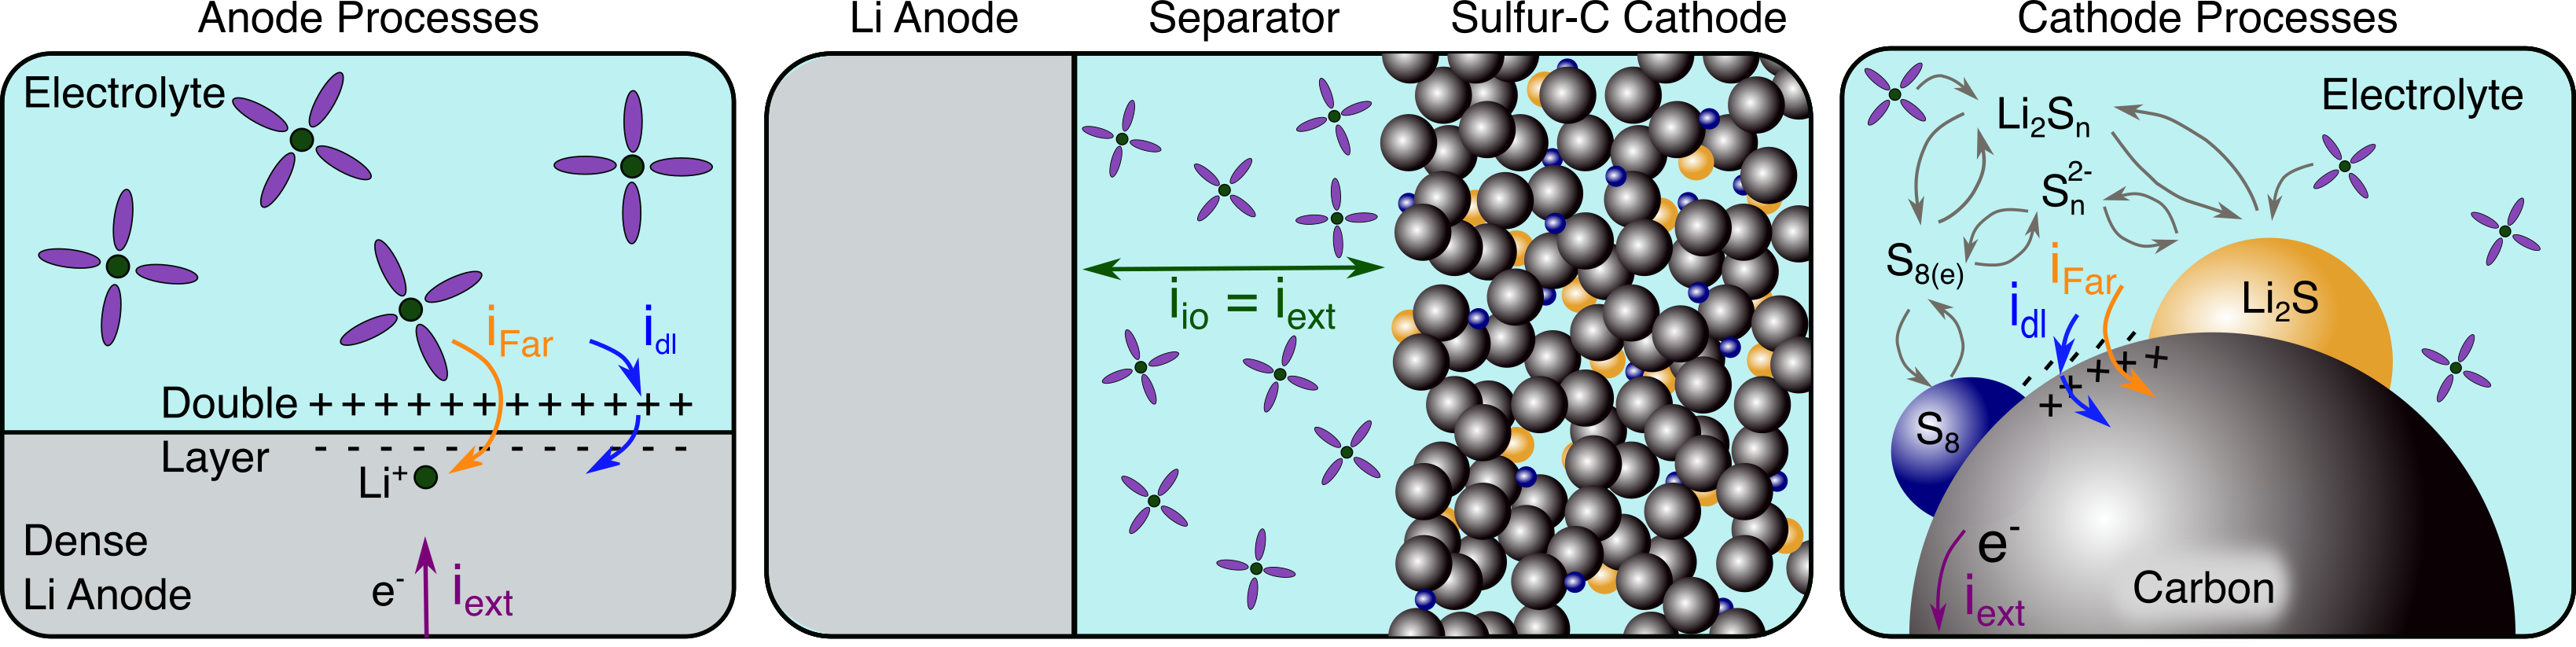
\includegraphics[width=0.75\textwidth]{Figure1_Simulation_Domain.png}
    \caption{Illustration of model domain and electrode processes.  The simulation includes an ideal Li metal anode, a porous electrolyte separator and a porous carbon cathode host, flooded with liquid electrolyte (1M LiTFSI in TEGDME). In the porous cathode, two chemical pathways between S$_8$ and Li$_2$S are examined, wherein the dissolved polysulfides are lithiated and non-lithiated, respectively.  Charge transfer reactions (Faradaic current and double-layer charging current) occur at the Li/electrolyte and carbon/electrolyte interfaces in the anode and cathode, respectively.}
    \label{fig:modeldomain}
\end{figure}
\subsection{Governing Equations}
The battery’s state at a given location is fixed by the following variables:

In the cathode:
\begin{itemize}
    \item $\varepsilon_{\rm S_8}$, volume fraction of solid sulfur (-)
	\item $\varepsilon_{\rm Li_2S}$, volume fraction of solid lithium sulfide (-)
	\item $C_{k,\,{\rm elyte}}$, molar concentration of species $k$ in the electrolyte phase $\left({\rm kmol}_k ~ {\rm m_{elyte}^{-3}}\right)$
	\item $\phi_{\rm carbon}$, the electric potential of the cathode carbon phase (V)
	\item $\phi_{\rm elyte}$, the electric potential of the electrolyte phase (V)
\end{itemize}

In the electrolyte separator:
\begin{itemize}
    \item $C_{k,\,{\rm elyte}}$, molar concentration of species $k$ in the electrolyte phase $\left({\rm kmol}_k ~ {\rm m_{elyte}^{-3}}\right)$
    \item $\phi_{\rm elyte}$, the electric potential of the electrolyte phase (V)
\end{itemize}

In the anode:
\begin{itemize}
    \item $C_{k,\,{\rm elyte}}$, molar concentration of species $k$ in the electrolyte phase $\left({\rm kmol}_k ~ {\rm m_{elyte}^{-3}}\right)$
    \item $\phi_{\rm elyte}$, the electric potential of the electrolyte phase (V)
    \item $\phi_{\rm Li}$, the electric potential of the metallic Li anode phase (V)
\end{itemize}

As mentioned above, the Li metal anode is modeled as a dense anode; however, to increase numerical stability of the model, a small ($5 ~ \mu \rm {m}$) buffer layer of electrolyte was added between the lithium/electrolyte interface and the separator.

The evolution of these variables during battery operation is predicted via governing equations derived from physically-based conservation equations for the mass, elements, and electrical charge:

\subsubsection{Solid Phase Volume Fractions}
For the cathode solid-phase end states --- solid sulfur (S$_8$) in the charged state and solid Li$_2$S in the discharged state --- constant mass density is assumed. As such, conservation of mass leads to the following for $\varepsilon_m$, the volume fraction of the solid phase $m$: 

\begin{equation}\label{eq:dEps_dt}
    \frac{\partial \varepsilon_m}{\partial t} = a_m\sum_{k,\,m} \overline{v}_k\dot{s}_k,
\end{equation}
where $\overline{v}_k$ is the constant molar volume (m$^3$ kmol$_k^{-1}$, equal to the molecular weight divided by the mass density) and $\dot{s}_k$ the molar production rate due to heterogeneous surface reactions (kmol$_k$ m$^{-2}$ s$^{-1}$) for species $k$, summed over all $k$ species in phase $m$.  The parameter $a_m$ is the volume-specific area (m$^{-1}$) of the reaction interface between the phase $m$ and the electrolyte.

\subsubsection{Electrolyte Species}
The molar concentration of the electrolyte species $k$ in the porous cathode and electrolyte separator varies with time due to chemical and electrochemical reactions, species transport, and the change in electrolyte volume fraction due to changing solid phase volume fractions. Conservation of mass and elements are combined to derive a differential equation for the evolution of the species molar concentrations $C_{k,\,{\rm elyte}}$  (kmol$_k$ m$_{\rm elyte}^{-3}$):
\begin{equation}\label{eq:dCkelyte_dt}
    \frac{\partial C_{k,\,{\rm elyte}}}{\partial t} = \frac{1}{\varepsilon_{\rm elyte}}\left(\sum_m a_m\dot{s}_{k,\,{\rm elyte}} + \dot{\omega}_{k,\,{\rm elyte}} - \nabla N_{k,\,{\rm elyte}}\right) - C_{k,\,{\rm elyte}}\frac{\partial \varepsilon_{\rm elyte}}{\partial t},
\end{equation}
where $\dot{\omega}_{k,\,{\rm elyte}}$ is the molar production rate of species $k$ due to homogeneous electrolyte phase reactions (kmol$_k$ m$_\mathrm{elyte}^{-3}$ s$^{-1}$) and $N_{k,\,{\rm elyte}}$ is the molar flux of electrolyte species $k$ (kmol$_k$ m$^{-2}$ s$^{-1}$). There are no surface reactions in the electrolyte separator ($a_m\dot{s}_{k,\,{\rm elyte}} = 0$), and homogeneous reactions are neglected throughout the modeling domain ($\dot{\omega}_{k,\,{\rm elyte}}=0$), for the present work. The rate of change of the electrolyte volume fraction $\left(\frac{\partial \varepsilon_{\rm elyte}}{\partial t}\right)$ is calculated as:
\begin{equation}\label{eq:dEpsElyte_dt}
    \frac{\partial \varepsilon_{\rm elyte}}{\partial t} = -\frac{\partial \varepsilon_{\rm S_8}}{\partial t} -\frac{\partial \varepsilon_{\rm Li_2S}}{\partial t},
\end{equation}
where the solid phase volume fraction rates of change are calculated as in eq.~\ref{eq:dEps_dt}, above. The electrolyte treatment makes two primary assumptions: that convective flux is negligible and that the total cell volume remains constant (i.e. the electrolyte is effectively compressible with no pressure effects). While convection is not directly modeled, increasing species concentration, e.g. in cathode regions with decreasing porosity, will lead to species diffusion toward low concentration / high porosity regions.  As shown in the results below, the species concentration gradients are relatively minor in most cases, and the foregoing assumptions have relative little impact.  Nonetheless, future work will implement species convection effects for a more robust model framework.

\subsubsection{Phase Electric Potentials}
 Within the cathode, the electrolyte and cathode carbon phase electric potentials are solved by applying conservation of charge and assuming charge neutrality. Charge neutrality in the electrolyte phase of a given volume implies that the sum of all currents into the volume equals zero:

 \begin{equation}\label{eq:ChargeCons_elyte}
     \nabla i_{\rm io} + i_{\rm Far,ca} + i_{\rm dl,ca} = 0,
 \end{equation}
where $i_{\rm io}$ is the ionic electrolyte phase current density ${\rm \left(A\,m^{-2}\right)}$, $i_{\rm Far,ca}$ is the local Faradaic charge transfer current per unit volume ${\rm \left(A\,m^{-3}\right)}$, and $i_{\rm dl,ca}$ is the local double-layer current per unit volume ${\rm \left(A\,m^{-3}\right)}$.  $i_{\rm Far,ca}$ and $i_{\rm dl,ca}$ are formulated such that positive current represents net positive charge transferred from the electrolyte phase to the solid electrode phase (lithium in the anode and carbon in the cathode), as illustrated schematically in Fig. \ref{fig:modeldomain}. 

%\begin{center}
%\begin{figure}
%    \centering
%    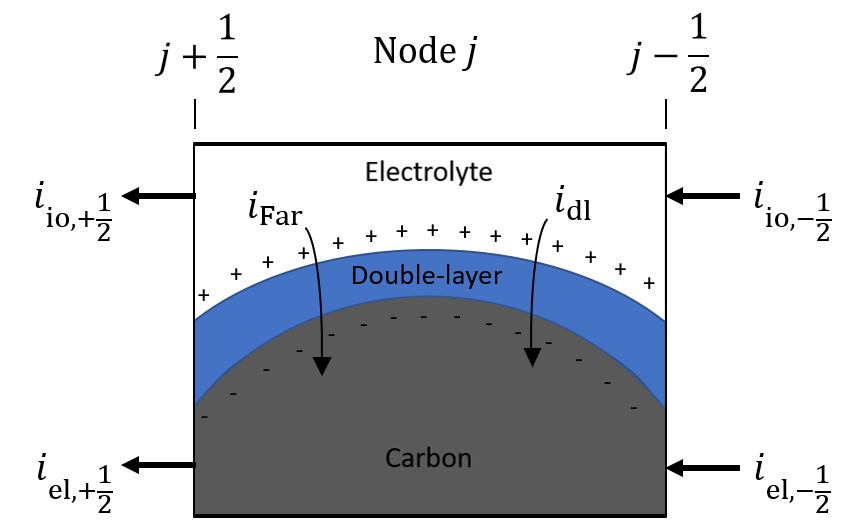
\includegraphics[width=\textwidth/2]{CurrentDiagram.png}
%    \caption{Caption}
%    \label{fig:currentdiagram}
%\end{figure}
%\end{center}

The ionic current in the electrolyte is a function of the species fluxes $N_{k,\,{\rm elyte}}$:
\begin{equation}\label{eq:i_io}
    i_{\rm io} = F\sum_{k,{\rm elyte}} z_kN_{k},
\end{equation}
where $F$ is Faraday's constant and $z_k$ is the elementary charge of species $k$. The double layer current, therefore, balances the residual of the sum of the remaining charge fluxes, transferring charge between the electrolyte bulk phase and the capacitive double layer at the electrolyte/electrode interface to maintain charge neutrality in the electrolyte bulk. Modeling the double layer as a capacitor with capacitance $C_{\rm dl}$ (F m$^{-2}$) links the rate of change of the double layer potential $\Delta \phi_{\rm dl}$ to the double-layer current:
\begin{equation}\label{eq:ddPhi_dt}
    \frac{\partial \Delta \phi_{\rm dl}}{\partial t} = \frac{i_{\rm dl}}{C_{\rm dl}\,a_{\rm dl}},
\end{equation}
where the double layer potential equals the difference between the electrode solid phase (`ed'--cathode or anode) and the bulk electrolyte (`elyte') phases:
\begin{equation}\label{eq:dPhi_dl}
    \Delta \phi_{\rm dl} = \phi_{\rm ed} - \phi_{\rm elyte}.
\end{equation}
Charge conservation and charge neutrality are also applied to each volume as a whole to yield:
\begin{equation}\label{eq:ChargeCons_tot}
    0 = \nabla i_{\rm io} + \nabla i_{\rm el},
\end{equation}
where $i_{\rm el}$ is the electronically conductive phase current density $\left({\rm A\,m^{-2}} \right)$, calculated via Ohm's Law. As documented below, $i_{\rm io}$ is a function of $C_{k,\,{\rm elyte}}$ and $\phi_{\rm elyte}$, while $i_{\rm el}$ is a function of $\phi_{\rm ca}$ only.  Eqs.~\ref{eq:ddPhi_dt}--~\ref{eq:ChargeCons_tot} therefore fix the electric potentials of the two phases throughout the domain. Eq.~\ref{eq:ddPhi_dt} represents a differential equation, integrated in time to solve the double layer potential $\Delta \phi_{\rm dl}$, which is used to calculate the $\phi_{\rm elyte}$ at any given time. Eq.~\ref{eq:ChargeCons_tot}, meanwhile, is an algebraic equation that must be satisfied at any point in time by the cathode carbon phase electric potentials. 

In the electrolyte separator, there is no electronic current, and so eq.~\ref{eq:ChargeCons_tot} reduces to:
\begin{equation}
    0 = \nabla i_{\rm io},
\end{equation}
with $i_{\rm io}$ calculated as in eq.~\ref{eq:i_io}. Boundary conditions therefore imply that $i_{\rm io} = i_{\rm ext}$, in the separator.

The anode is modeled as a dense Li foil, and as such the electric potential of the anode is resolved via a capacitive double layer at the electrolyte separator--anode boundary.  Charge neutrality in the anode requires that all currents sum to zero:
\begin{equation}\label{eq:ChargeConsAnode}
    i_{\rm ext} + i_{\rm Far,\,an} + i_{\rm dl,\,an} = 0,
\end{equation}
where all currents represent positive charge delivered to the bulk Li anode.  $i_{\rm ext}$ represents the user-specific external current (positive current corresponds to battery discharge).  As with the cathode, $i_{\rm dl}$ is used to calculate the rate of change of the anode--electrolyte double layer potential, via eq.~\ref{eq:ddPhi_dt}.


\subsection{Process Variables: Reaction and Transport Rate Calculations}

The charge-transfer reactions are evaluated using mass action kinetics and are handled by \textsc{Cantera}. The \textsc{Cantera} input file allows user specification of Arrhenius parameters (pre-exponential $A$, temperature exponent $b$, and activation energy $E_{\rm a}$) for the forward rate coefficient:
\begin{equation}\label{eq:k_fwd_echem}
    k_{\rm f} = AT^b\exp\left(-\frac{E_{\rm a}}{RT}\right)\exp\left(-\sum_k\frac{\beta\nu_kz_k\phi_k}{RT}\right).
\end{equation}
Here, $R$ is the universal gas constant, $T$ the temperature, $\beta$ the charge-transfer symmetry factor, and $\nu_k$, $z_k$, and $\phi_k$ are the net stoichiometric coefficient, elementary charge, and electric potential of the phase for species $k$, respectively.  For non-charge-transfer reactions, the electric potential summation evaluates to zero, and typical Arrhenius rate coefficients are recovered.  The reverse rate coefficient $k_{\rm r}$ for the same reaction is calculated as the reaction's equilibrium coefficient, divided by the forward rate coefficient, to maintain thermodynamic consistency \cite{DeCaluwe_2018}.

For a reaction $i$, the net rate of progress $\dot{q}_i$ is
\begin{equation}\label{eq:rop_net}
    \dot{q}_i = k_{{\rm f},i}\prod_k C_{{\rm ac},\,k}^{\nu^\prime_{k,i}} -  k_{{\rm r},i}\prod_k C_{{\rm ac},\,k}^{\nu^{\prime\prime}_{k,i}},
\end{equation}
where $\nu^\prime_{k,i}$ and  $\nu^{\prime\prime}_{k,i}$ are the forward and reverse stoichiometric coefficients for species $k$ in reaction $i$, respectively, and $C_{{\rm ac},\,K}$ is the ``activity concentration'' for species $k$ (equal to the molar density times the activity coefficient).  Finally, the net production rate for a given species due to a set of reactions ($\dot{s}_k$ or $\dot{\omega}_k$, above; we will use $\dot{s}_k$, here, for demonstration purposes) is:
\begin{equation}\label{eq:net_prod_rate}
    \dot{s}_k = \sum_i \nu_{k,i}\dot{q}_i,
\end{equation}
where $\nu_{k,i}=\nu^{\prime\prime}_{k,i} - \nu^{\prime}_{k,i}$ is the net stoichiometric coefficient for species $k$ in reaction $i$.

Transport rate calculations for electrolyte species use the Nernst-Poisson-Planck formulation and the dilute solution approximation:
\begin{equation}\label{eq:PNP}
    N_{k,{\rm elyte}} = -D_k^{\rm eff}\left(\nabla C_k + C_k\frac{z_kF}{RT}\nabla \phi_{\rm elyte}\right),
\end{equation}
where $C_k$ is taken at the interface between adjacent volumes (via weighted averaging of the volume-center concentrations) and $\nabla C_k$ uses the finite difference in volume-center concentrations. $D^{\rm eff}_k$ the effective diffusion coefficient, which incorporates the dynamically-varying local microstructure is:
\begin{equation}\label{eq:Dk_eff}
    D^{\rm eff}_k = \frac{\varepsilon_{\rm elyte}}{\tau_{\rm fac}}D^\circ_k = D^\circ_k\varepsilon_{\rm elyte}^{1.5}
\end{equation}
where the bulk diffusion coefficient (absent microstructure impacts) is $D^\circ_k$, and where we replace the local tortuosity factor $\tau_{\rm fac}$ with a simple Bruggeman correlation, $n_{\rm Bruggeman} = -0.5$ \cite{TJADEN201644}.  Although eq.~\ref{eq:PNP} can accommodate the more accurate concentrated solution theory (CST) \cite{Kupper_2016}, the CST framework requires significant alteration to accomodate the multiple charged species in the Li-S system \cite{mukherjee2018}, and is left for future work. While this model focuses on the thermochemical effects present due to electrolyte concentrations, it has also been shown that electrolyte concentrations can impact transport properties \cite{Zhang2015, Robinson_2021}; however, implementation of these aspects is left to future work.

\subsection{Initial Conditions and Geometric Parameters}
One novel feature of this model is the use of physically derived geometric parameters to directly link model microstructural parameters to  battery design and fabrication parameters from reported experiments. Here, we describe the derivation of  microstructural parameters from a small number of experimental/cell fabrication variables and physical constants:
\begin{itemize}
    \item $m^{\prime\prime,\circ}_{\rm S_8}$, the initial mass loading of sulfur (kg m$^{-2}$)
    \item $m^\circ_{\rm S_8}$, the initial bulk mass of sulfur (kg)
    \item $\omega^\circ_m$, the weight percent of each phase $m$ (kg$_m$ kg$^{-1}_{\rm tot}$)
    \item $H_{\rm ca}$, the cathode thickness (m)
    \item $\rho_m$, the mass density of phase $m$, (kg$_m$ m$^{-3}_m$)
\end{itemize}
These input parameters allow calculation of the initial volume fraction of solid phases:
\begin{equation}\label{eq:esp_S8_o}
    \varepsilon_{\rm S_8}^\circ = \frac{m^{\prime\prime,\circ}_{\rm S_8}}{\rho_{\rm S_8} H_{\rm ca}}
\end{equation}
\begin{equation}\label{eq:m_solid_o}
    m^{\prime\prime,\circ}_{\rm solid} = \frac{m^{\prime\prime,\circ}_{\rm S_8}}{\omega^\circ_{\rm S_8}}
\end{equation}
\begin{equation}\label{eq:eps_carbon_o}
    \varepsilon^\circ_{\rm carbon} = \frac{ m^{\prime\prime,\circ}_{\rm solid}\omega^\circ_{\rm carbon}}{\rho_{\rm carbon}H_{\rm ca}}
\end{equation}
\begin{equation}\label{eq:eps_elyte_o}
    \varepsilon^\circ_{\rm elyte} = 1 - \varepsilon^\circ_{\rm S_8} - \varepsilon^\circ_{\rm carbon} - \varepsilon^\circ_{\rm Li_2S}
\end{equation}
The initial Li$_2$S is assumed very small ($\varepsilon^{o}_{\rm{Li}_2\rm{S}} = 10^{-5}$) and all solid phases are assumed to have constant mass density $\rho_m$.

Assuming hemispherical particles of active end products (S$_8$ and Li$_2$S) in the cathode, the volume-specific surface area of the active phases is derived using the following variables:
\begin{itemize}
    \item $r_m$, radius of the representative hemisphere of phase $m$ (m)
    \item $a_m$, volume specific surface area of phase $m$ (m$^2_m$ m$^{-3}_{\rm tot}$)
    \item $n_m$, the number of hemispheres of phase $m$, per unit volume (m$^{-3}_{\rm tot}$)
\end{itemize}
Where $n_m$ is constant and $r_m$ varies as $\varepsilon_m$ changes.

The exposed surface area per unit volume of a hemisphere being equal to $3/r_m$, the total exposed surface area for phase $m$ per unit total volume of electrode is:
\begin{equation}\label{eq:area_per_vol_m_1}
    a_m = \frac{3\varepsilon_m}{r_m}
\end{equation}
This expression is reformulated, so as to be a function of only the state variable $\varepsilon_m$ and the (assumed constant) number of particles $n_m$:
\begin{equation}\label{eq:area_per_vol_m_2}
    a_m = 2\pi n_m\left(\frac{3\varepsilon_m}{2\pi n_m}\right)^{^2/_3}
\end{equation}
The active carbon surface area is calculated by assuming an intrinsic carbon surface area and then subtracting the area covered by the active phase hemispheres at any given time:
\begin{equation}\label{eq:a_carbon}
    a_{\rm carbon} = a^\circ_{\rm carbon} - \sum_m n_m\pi r_m^2
\end{equation}

The source code for the model is available via GitHub \cite{LiSCode} as well as the data, figures, and manuscript of this work \cite{LiSPaper}


%===============================================================%
%                      RESULTS
%===============================================================%
\section{Results}
Model results are presented below for four separate thermo-kinetic mechanisms. Two are original to this work, developed in-house as an extension of previous continuum-based mechanisms \cite{Kumaresan_2008, Neidhardt_2012}, and are detailed in Tables~\ref{tab:non_lithiated_thermo}--\ref{tab:lithiated_kinetics}.
\begin{itemize}
    \item `Non-lithiated polysulfides': This mechanism follows the typical form from previous continuum simulations, including a linear cascade of polysulfides S$^{2-}_n$ of decreasing order $n$.
    \item `Lithiated polysulfides': This mechanism includes the same species and reactions as the `non-lithiated' mechanism, but with all intermediates as lithiated, charge-neutral polysulfides Li$_2$S$_n$.
\end{itemize}

%---------------------------------------
% TABLE OF LITHIATED AND NON-LITHIATED PARAMETERS
%---------------------------------------

\begin{table}[h!]
\begin{center}
 \begin{tabular}{cccc}
 \hline\hline
 Species & ${h}^\circ_k ~ \left(\mathrm{kJ} ~ \mathrm{mol}^{-1}\right)$  & ${D}^\circ_k ~ \left(\mathrm{m}^2 ~ \mathrm{s}^{-1}\right)$ & ${C}^0_{k} ~ \left(\mathrm{kmol} ~ \mathrm{m}^{-3}\right)$ \\
 \hline
 \multicolumn{4}{l}{\bf Solid Cathode Species}\\
 $\mathrm{S}_8(\mathrm{s})$ & 0.0 &  &  \\
 $\mathrm{Li}_2\mathrm{S}(\mathrm{s})$ & -1112.48  & &  \\
 \multicolumn{4}{l}{\bf Liquid Electrolyte Species}\\
 $\mathrm{S}_8(\mathrm{e})$ & 16.1  & $1 \times 10^{-11}$ & $1.943 \times 10^{-2}$ \\
 $\mathrm{S}_8^{2-}$ & -450.78  & $6 \times 10^{-11}$ & $1.821 \times 10^{-4}$ \\
 $\mathrm{S}_6^{2-}$ & -445.15  & $6 \times 10^{-11}$ & $3.314 \times 10^{-4}$ \\
 $\mathrm{S}_4^{2-}$ & -433.14  & $1 \times 10^{-10}$ & $2.046 \times 10^{-5}$ \\
 $\mathrm{S}_2^{2-}$ & -401.82 & $1 \times 10^{-10}$ & $5.348 \times 10^{-10}$ \\
 $\mathrm{S}^{2-}$ & -383.27  & $1 \times 10^{-10}$ & $8.456 \times 10^{-13}$ \\
 $\mathrm{Li}^+$ & -278.0 & $1 \times 10^{-10}$ & $1.024$ \\
 $\mathrm{TFSI}^-$ & 0.0 &  $4 \times 10^{-10}$ & $1.0229$ \\
 $\mathrm{TEGDME}$ & 0.0 &  $1 \times 10^{-12}$ & $1.023 \times 10^{1}$ \\
 \multicolumn{4}{l}{\bf Solid Anode Species}\\
  $\mathrm{Li}(\mathrm{s})$ & 0.0 & &  \\
 \hline\hline
\end{tabular}
\caption{Species parameters and initial conditions for the `non-lithiated polysulfide' mechanism. For species $k$, $h^\circ_k$ is the standard-state molar enthalpy, $s^\circ_k$ the standard-state molar entropy, $D^\circ_k$ the bulk-phase diffusion coefficient, and $C^0_k$ is the initial molar concentration. For the current isothermal model, $s^\circ_k$ was assumed as 0.0 kJ mol$^{-1}$ K$^{-1}$, and $h^\circ_k$ was used to fit the species chemical potentials to match experimental discharge curves.}
\label{tab:non_lithiated_thermo}
\end{center}
\end{table}

\begin{table}[h!]
\begin{center}
\begin{tabular}{ clc } 
 \hline\hline
 Reaction & Forward rate constant & Units \\ 
 \hline
 \multicolumn{1}{l}{\bf Sulfur/electrolyte interface} & &   \\
 $\mathrm{S}_8(\mathrm{s}) \rightleftharpoons \mathrm{S}_8(\mathrm{e})$ & $1.9 \times 10^{-2}$ & $ - $ \\ 
 \hline
 \multicolumn{1}{l}{\bf Carbon/electrolyte interface} & & \\
 $\frac{1}{2} ~ \mathrm{S}_8(\mathrm{e}) + \mathrm{e}^- \rightleftharpoons \frac{1}{2} ~ \mathrm{S}_8^{2-}$ & $8.725 \times 10^{16}$ & $\mathrm{kmol}^{0.5} ~ \mathrm{m}^{-0.5} ~ \mathrm{s}^{-1}$   \\
 
 $\frac{3}{2} ~ \mathrm{S}_8^{2-} + \mathrm{e}^- \rightleftharpoons 2 ~ \mathrm{S}_6^{2-}$ & $4.331 \times 10^{17}$ & $\mathrm{kmol}^{-0.5} ~ \mathrm{m}^{2.5} ~ \mathrm{s}^{-1}$  \\
 
  $\mathrm{S}_6^{2-} + \mathrm{e}^- \rightleftharpoons \frac{3}{2} ~ \mathrm{S}_4^{2-}$ & $3.193 \times 10^{15}$ & $\mathrm{m}^{1} ~ \mathrm{s}^{-1}$  \\
 
  $\frac{1}{2} ~ \mathrm{S}_4^{2-} + \mathrm{e}^- \rightleftharpoons \mathrm{S}_2^{2-}$ & $2.375 \times 10^{12} $ & $ \mathrm{kmol}^{0.5} ~ \mathrm{m}^{-0.5} ~ \mathrm{s}^{-1}$  \\
 
  $\frac{1}{2} ~ \mathrm{S}_2^{2-} + \mathrm{e}^- \rightleftharpoons \mathrm{S}^{2-}$ &$8.655 \times 10^{13} $ & $ \mathrm{kmol}^{0.5} ~ \mathrm{m}^{-0.5} ~ \mathrm{s}^{-1}$  \\
 \hline
 \multicolumn{1}{l}{\bf Li$_2$S(s)/electrolyte interface} & &  \\
  $2 ~ \mathrm{Li}^+ + \mathrm{S}^{2-} \rightleftharpoons \mathrm{Li}_2\mathrm{S}(\mathrm{s})$ & $1.075 $ & $ \mathrm{kmol}^{-2} ~ \mathrm{m}^{7} ~ \mathrm{s}^{-1}$  \\
 \hline
 \multicolumn{1}{l}{\bf Li(s)/electrolyte interface} & &  \\
  $\mathrm{Li}(\mathrm{s}) \rightleftharpoons \mathrm{Li}^+ + \mathrm{e}^-$ & $3.0 \times 10^{-8} $ & $\mathrm{kmol} ~ \mathrm{m}^{-2} ~ \mathrm{s}^{-1}$  \\
 \hline\hline
 \end{tabular}
 \caption{Kinetic parameters for the `non-lithiated polysulfide' mechanism in this work.}
\label{tab:non_lithiated_kinetics}
\end{center}
 \end{table}
 
\begin{table}[h!]
\begin{center}
 \begin{tabular}{cccc}
 \hline\hline
 Species & ${h}^\circ_k ~ \left(\mathrm{kJ} ~ \mathrm{mol}^{-1}\right)$  & ${D}^\circ_k ~ \left(\mathrm{m}^2 ~ \mathrm{s}^{-1}\right)$ & ${C}^\circ_{k} ~ \left(\mathrm{kmol} ~ \mathrm{m}^{-3}\right)$ \\
 \hline
 \multicolumn{4}{l}{\bf Solid Cathode Species}\\
 $\mathrm{S}_8(\mathrm{s})$ & 0.0  &  &  \\
 $\mathrm{Li}_2\mathrm{S}(\mathrm{s})$ & -1112.48 &  &  \\
 \multicolumn{4}{l}{\bf Liquid Electrolyte Species}\\
 $\mathrm{S}_8(\mathrm{e})$ & 16.1 & $1 \times 10^{-11}$ & $1.943 \times 10^{-2}$ \\
 $\mathrm{Li}_2\mathrm{S}_8$ & -1006.78  & $6 \times 10^{-11}$ & $1.821 \times 10^{-4}$ \\
 $\mathrm{Li}_2\mathrm{S}_6$ & -1004.15  & $6 \times 10^{-11}$ & $3.314 \times 10^{-4}$ \\
 $\mathrm{Li}_2\mathrm{S}_4$ & -994.14  & $1 \times 10^{-10}$ & $2.046 \times 10^{-5}$ \\
 $\mathrm{Li}_2\mathrm{S}_2$ & -963.82 & $1 \times 10^{-10}$ & $5.348 \times 10^{-10}$ \\
 $\mathrm{Li}_2\mathrm{S}(\mathrm{e})$ & -941.27  & $1 \times 10^{-10}$ & $8.456 \times 10^{-13}$ \\
 $\mathrm{Li}^+$ & -278.0 & $1 \times 10^{-10}$ & $1.024$ \\
 $\mathrm{TFSI}^-$ & 0.0  & $4 \times 10^{-10}$ & $1.024$ \\
 $\mathrm{TEGDME}$ & 0.0 & $1 \times 10^{-12}$ & $1.023 \times 10^{1}$ \\
 \multicolumn{4}{l}{\bf Solid Anode Species}\\
 $\mathrm{Li}(\mathrm{s})$ & 0.0 & &  \\
 \hline\hline
\end{tabular}
\caption{Species parameters and initial conditions for the `lithiated polysulfide' mechanism. For species $k$, $h^\circ_k$ is the standard-state molar enthalpy, $s^\circ_k$ the standard-state molar entropy, $D^\circ_k$ the bulk-phase diffusion coefficient, and $C^0_k$ is the initial molar concentration. For the current isothermal model, $s^\circ_k$ was assumed as 0.0 kJ mol$^{-1}$ K$^{-1}$, and $h^\circ_k$ was used to fit the species chemical potentials to match experimental discharge curves.}
\label{tab:lithiated_thermo}
\end{center}
\end{table}

\begin{table}[h!]
\begin{center}
\begin{tabular}{ clc } 
 \hline\hline
 Reaction & Forward rate constant & Units \\ 
 \hline
 \multicolumn{1}{l}{\bf Sulfur/electrolyte interface} & &   \\
 $\mathrm{S}_8(\mathrm{s}) \rightleftharpoons \mathrm{S}_8(\mathrm{e})$  & $1.9 \times 10^{-2}$ & - \\ 
 \hline
 \multicolumn{1}{l}{\bf Carbon/electrolyte interface} & & \\
 $\frac{1}{2} ~ \mathrm{S}_8(\mathrm{e}) + \mathrm{Li}^+ + \mathrm{e}^- \rightleftharpoons \frac{1}{2} ~ \mathrm{Li}_2\mathrm{S}_8$ & $8.725 \times 10^{16}$ & $\mathrm{kmol}^{-0.5} ~ \mathrm{m}^{2.5} ~ \mathrm{s}^{-1}$   \\
 
 $\frac{3}{2} ~ \mathrm{Li}_2\mathrm{S}_8 + \mathrm{Li}^+ + \mathrm{e}^- \rightleftharpoons 2 ~ \mathrm{Li}_2\mathrm{S}_6$ & $4.331 \times 10^{17}$ & $\mathrm{kmol}^{-1.5} ~ \mathrm{m}^{5.5} ~ \mathrm{s}^{-1}$  \\
 
 $\mathrm{Li}_2\mathrm{S}_6 + \mathrm{Li}^+ + \mathrm{e}^- \rightleftharpoons \frac{3}{2} ~ \mathrm{Li}_2\mathrm{S}_4$ & $3.193 \times 10^{15}$ & $\mathrm{kmol}^{-1} ~ \mathrm{m}^{4} ~ \mathrm{s}^{-1}$  \\
 
 $\frac{1}{2} ~ \mathrm{Li}_2\mathrm{S}_4 + \mathrm{Li}^+ + \mathrm{e}^- \rightleftharpoons  \mathrm{Li}_2\mathrm{S}_2$ & $2.375 \times 10^{12}$ & $ \mathrm{kmol}^{-0.5} ~ \mathrm{m}^{2.5} ~ \mathrm{s}^{-1}$  \\
 
 $\frac{1}{2} ~ \mathrm{Li}_2\mathrm{S}_2 + \mathrm{Li}^+ + \mathrm{e}^- \rightleftharpoons  \mathrm{Li}_2\mathrm{S}(\mathrm{e})$ & $8.655 \times 10^{13}$ & $ \mathrm{kmol}^{-0.5} ~ \mathrm{m}^{2.5} ~ \mathrm{s}^{-1}$  \\
 \hline
 \multicolumn{1}{l}{\bf Li$_2$S(s)/electrolyte interface} & &  \\
 $\mathrm{Li}_2\mathrm{S}(\mathrm{e}) \rightleftharpoons \mathrm{Li}_2\mathrm{S}(\mathrm{s})$ & $1.075 $ & $ \mathrm{m} ~ \mathrm{s}^{-1}$  \\
 \hline
 \multicolumn{1}{l}{\bf Li(s)/electrolyte interface} & & 
\\
 $\mathrm{Li}(\mathrm{s}) \rightleftharpoons \mathrm{Li}^+ + \mathrm{e}^-$ & $3.0 \times 10^{-8}$ & $\mathrm{kmol} ~ \mathrm{m}^{-2} ~ \mathrm{s}^{-1}$  \\
 \hline\hline
 \end{tabular}
 \caption{Kinetic parameters for the `lithiated polysulfide' mechanism in this work.}
\label{tab:lithiated_kinetics}
\end{center}
 \end{table}
For future studies that incorporate both lithiated and non-lithiated pathways, developing combined thermo-kinetic mechanisms will require estimates for all of the parameters in Tables~\ref{tab:non_lithiated_thermo}--\ref{tab:lithiated_kinetics}, upwards of 50 parameters. Even with detailed, \textit{operando} physical chemistry validation data, rigorously fitting this many parameters via a continuum-level model is not realistic.  Rather, simulations will need to leverage atomistic calculations to provide thermo-kinetic parameter estimates. To demonstrate the adoption of atomistic mechanisms, we also show results using thermodynamics adopted from studies by Assary, \textit{et al.}~\cite{assary2014}, and Kuz'mina, \textit{et al.}~\cite{kuzmina2019}.  Adopted parameters for these mechanisms are provided in Supplementary Tables~1 and 2.  The thermodynamic parameters are adopted wholesale from selected species from these references, while the kinetic parameters are hand-fitted to agree with experimental data.

The results below present simulation results for two separate studies.  First, simulations use an initial cathode porosity of 85\% to match experimental data presented by Andrei,\textit{ et al.}~\cite{ANDREI2018469} This allows for validation of model results and a detailed comparison of the four mechanisms described above.  From these results, the `lithiated polysulfide' mechanism developed as part of this work is chosen as providing the best fit to data. The remaining results use this mechanism to demonstrate the use of the detailed chemical model framework as a Li-S battery design tool. We explore the impact of varying the electrolyte/sulfur (E/S) ratio on the battery performance and dissolved polysulfide concentrations. 
%---------------------------------------
% TABLE OF ASSARY AND KUZMINA PARAMETERS
%---------------------------------------
% \begin{table}[h!]
% \begin{center}
%  \begin{tabular}{ccccccc}
%  \hline \hline
%  Species & \multicolumn{2}{c}{${h}^\circ_k ~ \left(\mathrm{kJ} ~ \mathrm{mol}^{-1} \right)$}& \multicolumn{2}{c}{${s}^\circ_k ~ \left(\mathrm{kJ} ~ \mathrm{mol}^{-1} ~ \mathrm{K}^{-1}\right)$} & ${D}^\circ_k ~ \left(\mathrm{m}^2 ~ \mathrm{s}^{-1}\right)$ &
%  $C^\circ_k$ $\left(\mathrm{kmol}~\mathrm{m}^{-3}\right)$ \\
%  \cmidrule(lr){2-3}\cmidrule(lr){4-5}
%  & Assary & Kuz'mina &Assary  & Kuz'mina  & &  \\
%  \hline
%  \multicolumn{6}{l}{\bf Solid Cathode Species}\\
%  $\mathrm{S}_8(\mathrm{s})$ & 0.0 & 0.0 & 0.0 & 0.0  \\
%  $\mathrm{Li}_2\mathrm{S}(\mathrm{s})$ & -1025.1& -929.1 & -26.1 & -81.0 & \\
%  \multicolumn{6}{l}{\bf Liquid Electrolyte Species}\\
%  $\mathrm{S}_8(\mathrm{e})$ & 16.1 & 16.1 & 0.0 & 0.0 & $1 \times 10^{-11}$ & $1.943 \times 10^{-4}$  \\
%  $\mathrm{Li}_2\mathrm{S}_8$ & -1403.7 & -1040.9 & -142.5 & -142.5 & $6 \times 10^{-11}$ & $1.821 \times 10^{-4}$ \\
%  $\mathrm{Li}_2\mathrm{S}_6$ & -1317.7 & -1032.7 & -3.8 & -117.0 & $6 \times 10^{-11}$ & $3.314 \times 10^{-6}$ \\
%  $\mathrm{Li}_2\mathrm{S}_4$ & -1341.9 & -1030.5 & -95.8 & -95.8 & $1 \times 10^{-10}$ & $2.046 \times 10^{-8}$ \\
%  $\mathrm{Li}_2\mathrm{S}_3$ & -1098.5 & -1103.3 & 75.4 & -93.8 & $1 \times 10^{-10}$ & $2.046 \times 10^{-10}$ \\
%  $\mathrm{Li}_2\mathrm{S}_2$ & -1082.2 & -1034.2 & 25.8 & -85.0 & $1 \times 10^{-10}$ & $5.348 \times 10^{-16^\mathrm{(a)}}$ \\
%  $\mathrm{Li}^+$ & -278.0 & -278.0 & 13.4 & 13.4 & $1 \times 10^{-10}$ & $1.024$ \\
%  $\mathrm{TFSI}^-$ & 0.0 & 0.0 & 0.0 & 0.0 & $4 \times 10^{-10}$ & $1.024$ \\
%  $\mathrm{TEGDME}$ & 0.0 & 0.0 & 0.0 & 0.0 & $1 \times 10^{-12}$ & $1.023 \times 10^{1}$ \\
%  \multicolumn{4}{l}{\bf Solid Anode Species}\\
%  $\mathrm{Li}(\mathrm{s})$ & 0.0 & 0.0 & 0.0 & 0.0 &  \\
%  \hline\hline
% \end{tabular}
% \caption{Thermodynamic parameters of mechanisms based on Assary \textit{et al.} \cite{assary2014} and Kuz'mina \textit{et al.}~\cite{kuzmina2019}For species $k$, $h^\circ_k$ is the standard-state molar enthalpy, $s^\circ_k$ the standard-state molar entropy, $D^\circ_k$ the bulk-phase diffusion coefficient, and $C^0_k$ is the initial molar concentration. For the current isothermal model, $s^\circ_k$ was assumed as 0.0 kJ mol$^{-1}$ K$^{-1}$, and $h^\circ_k$ was used to fit the species chemical potentials to match experimental discharge curves. (a) The initial concentration for $\mathrm{Li}_2\mathrm{S}_2$ in the Kuz'mina mechanism was $5.348 \times 10^{-13} ~ \mathrm{kmol} ~ \mathrm{m}^{-3}$}
% \label{tab:atomistic_thermo}
% \end{center}
% \end{table}

% \begin{table}[h!]
% \begin{center}
% \begin{tabular}{ cccc } 
%  \hline\hline
%  Reactions & \multicolumn{2}{c}{Forward rate constant} & Units \\ 
%  \cmidrule(lr){2-3}
%  & Assary & Kuz'mina & \\
%  \hline
%  \multicolumn{4}{l}{\bf Sulfur/electrolyte interface}   \\
%  $\mathrm{S}_8(\mathrm{s}) \rightleftharpoons \mathrm{S}_8(\mathrm{e})$ &  $1.0 \times 10^{-6}$ &$1.0 \times 10^{-4}$ & $\mathrm{kmol} ~ \mathrm{m}^{-2} ~ \mathrm{s}^{-1}$ \\ 
%  \hline
%  \multicolumn{4}{l}{\bf Carbon/electrolyte interface}   \\
%  $\mathrm{S}_8(\mathrm{e}) + 2 ~ \mathrm{Li}^+ + 2 ~ \mathrm{e}^- \rightleftharpoons \mathrm{Li}_2\mathrm{S}_8$ & $1.0 \times 10^{13}$ & $1.0 \times 10^{13}$ & $\mathrm{kmol}^{-2} ~ \mathrm{m}^{7} ~ \mathrm{s}^{-1}$   \\
%  $\mathrm{Li}_2\mathrm{S}_8 + 2 ~ \mathrm{Li}^+ + 2 ~ \mathrm{e}^- \rightleftharpoons  \mathrm{Li}_2\mathrm{S}_6 + \mathrm{Li}_2\mathrm{S}_2$ & $1.0 \times 10^{11}$ & $2.0 \times 10^{11}$ & $\mathrm{kmol}^{-2} \mathrm{m}^{7} ~ \mathrm{s}^{-1}$  \\
%  $\mathrm{Li}_2\mathrm{S}_6 + 2 ~ \mathrm{Li}^+ + 2 ~ \mathrm{e}^- \rightleftharpoons \mathrm{Li}_2\mathrm{S}_4 + \mathrm{Li}_2\mathrm{S}_2$ & $1.0 \times 10^{8}$ & $5.0 \times 10^{7}$ & $\mathrm{kmol}^{-2} ~ \mathrm{m}^{7} ~ \mathrm{s}^{-1}$  \\
%  $\mathrm{Li}_2\mathrm{S}_8 + 2 ~ \mathrm{Li}^+ + 2 ~ \mathrm{e}^- \rightleftharpoons  2 ~ \mathrm{Li}_2\mathrm{S}_4$ & $1.0 \times 10^{7}$ & $1.0 \times 10^{7}$ & $\mathrm{kmol}^{-2} ~ \mathrm{m}^{7} ~ \mathrm{s}^{-1}$  \\
%  \hline
%  \multicolumn{4}{l}{\bf Li$_2$S(s)/carbon/electrolyte boundary}  \\
%  $\mathrm{Li}_2\mathrm{S}_4 + 2 ~ \mathrm{Li}^+ + 2 ~ \mathrm{e}^- \rightleftharpoons  \mathrm{Li}_2\mathrm{S}_3 + \mathrm{Li}_2\mathrm{S}(\mathrm{s})$ &  $1.0 \times 10^{7}$ & $1.0 \times 10^{7}$ & $\mathrm{kmol}^{-2} ~ \mathrm{m}^{7} ~ \mathrm{s}^{-1}$  \\
%  $\mathrm{Li}_2\mathrm{S}_3 + 2 ~ \mathrm{Li}^+ + 2 ~ \mathrm{e}^- \rightleftharpoons \mathrm{Li}_2\mathrm{S}_2 + \mathrm{Li}_2\mathrm{S}(\mathrm{s})$ & -- &  $1.0 \times 10^{7}$ & $\mathrm{kmol}^{-2} ~ \mathrm{m}^{7} ~ \mathrm{s}^{-1}$ \\
%  $\mathrm{Li}_2\mathrm{S}_2 + 2 ~ \mathrm{Li}^+ + 2 ~ \mathrm{e}^- \rightleftharpoons 2 ~ \mathrm{Li}_2\mathrm{S}(\mathrm{s})$ & -- & $1.0 \times 10^{3}$ & $\mathrm{kmol}^{-2} ~ \mathrm{m}^{7} ~ \mathrm{s}^{-1}$ \\
%  \hline
%  \multicolumn{4}{l}{\bf Li$_2$S(s)/electrolyte interface} \\
%  $ 2 ~ \mathrm{Li}_2\mathrm{S}_3 \rightarrow \mathrm{Li}_2\mathrm{S}_2 + \frac{1}{4} ~ \mathrm{S}_8(\mathrm{e})$ & \ $1.0 \times 10^{-2}$ & -- & $\mathrm{kmol}^{-1} ~ \mathrm{m}^{4} ~ \mathrm{s}^{-1}$  \\
%  $\mathrm{Li}_2\mathrm{S}_2 \rightarrow 2 ~ \mathrm{Li}_2\mathrm{S}(\mathrm{s}) + \frac{1}{4} ~ \mathrm{S}_8(\mathrm{e})$ &  $1.0 \times 10^{-5}$ & -- & $\mathrm{m} ~ \mathrm{s}^{-1}$\\
%  \hline
%  \multicolumn{4}{l}{\bf Li(s)/electrolyte interface}  \\
%  $\mathrm{Li}(\mathrm{s}) \rightleftharpoons \mathrm{Li}^+ + \mathrm{e}^-$ & $1.0 \times 10^{3}$ & $1.0 \times 10^{3}$ & $\mathrm{kmol} ~ \mathrm{m}^{-2} ~ \mathrm{s}^{-1}$  \\
%  \hline\hline
%  \end{tabular}
% \caption{Kinetic parameters for atomistic mechanisms based on Assary \textit{et al.} \cite{assary2014} and Kuz'mina \textit{et al.} \cite{kuzmina2019}}
% \label{tab:atomistic_kinetics}
% \end{center}
% \end{table}
\subsection{Model Validation}
During discharge, Li$_2$S formation proceeds via heterogeneous nucleation and growth of Li$_2$S particles at carbon surfaces, with the nature of the precipitate dependent on the C-rate~\cite{REN2016115}. At low C-rates, fewer Li$_2$S nucleates form, which grow larger as discharge proceeds. Conversely, at high C-rates Li$_2$S tends to form a greater number of smaller nuclei, which can form a passivating film in extreme cases. The nature of the nucleation and growth phenomena therefore impacts the surface area evolution and the porosity during discharge. In order to capture this C-rate dependence of nucleation density within a standard continuum-model framework, we developed a semi-empirical function to relate the applied C-rate to the nucleation density $n_m$ of the solid Li$_2$S in the cathode:
\begin{equation}\label{eq:li2s_nucl}
    n_m = 5 \times 10^{13} ~ \exp \left( 2.4221 \times C \right)
\end{equation}
where $C$ is the C-rate input into the model file. For the atomistic mechanisms (Assary, \textit{et al.} and Kuz'mina, \textit{et al.}), the function is $6 \times 10^{13} ~ \exp \left( 1.8966 \times C \right)$. Future work will directly implement heterogeneous nucleation and growth kinetics, for a physics-based understanding of solid phase morphology as a function of operating conditions. 

\begin{figure}[b!]
    \centering
    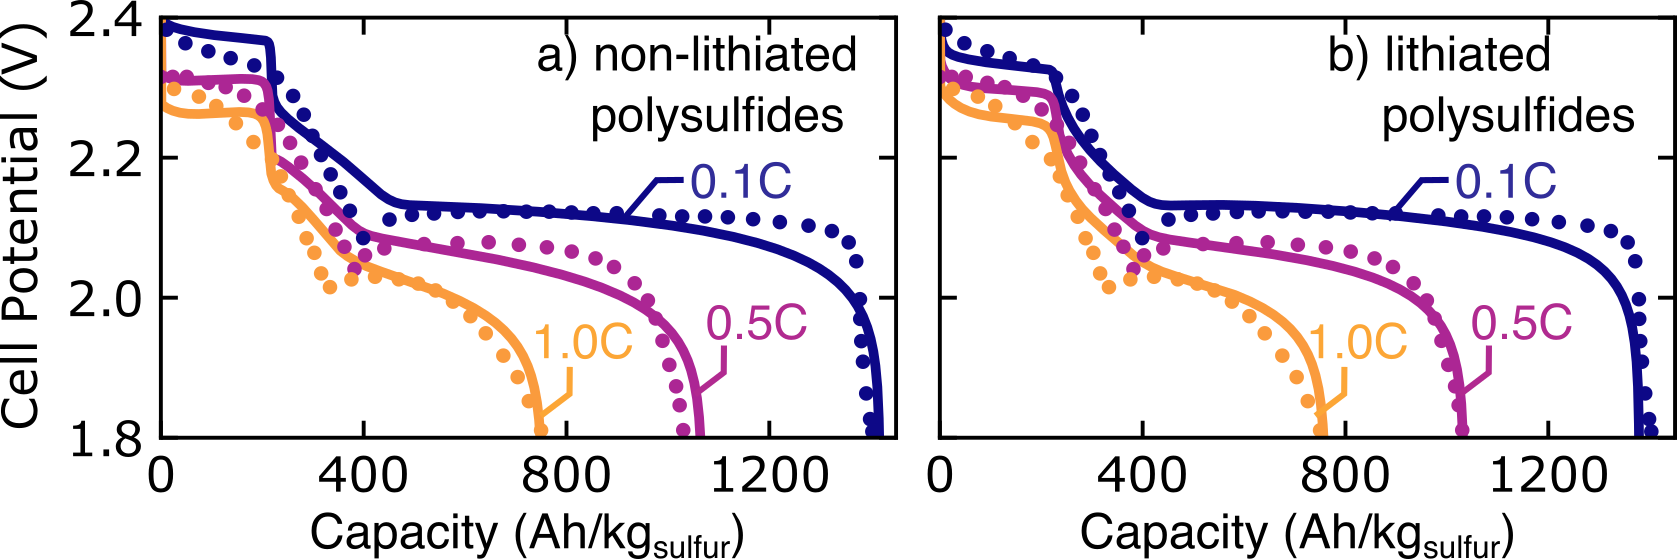
\includegraphics[width=\textwidth]{Figures/Figure2_validation.png}
    \caption{Validation of the (a) `non-lithiated' and (b) `lithiated' polysulfide mechanisms to experimental data taken from Andrei \textit{et al.} \cite{ANDREI2018469} at 0.1C, 0.5C, and 1C discharge.}
    \label{fig:model_validation}
\end{figure}

The model is validated by fitting the thermo-kinetic parameters for the `non-lithiated' and `lithiated' cascade mechanism (i.e., Tables~\ref{tab:non_lithiated_thermo}--\ref{tab:lithiated_kinetics}) against data from Andrei, \textit{et al.}~\cite{ANDREI2018469}, taken at C-rates of 0.1C, 0.5C, and 1.0C. Fitting results, presented in Figure \ref{fig:model_validation}, show that both models capture the discharge capacity rate dependence and major features of the discharge profiles. The mechanism using lithiated polysulfides provides a slightly better fit, particularly with regard to the shape of the lower voltage plateau. The two mechanisms are compared in greater detail, in the following section.  %All mechanism parameters for these two forms can be found in table \ref{cascadekineticsandthermo}. 

It is worth noting that, while the lithiated form of this mechanism produces good aggreement with the data at 0.1C, it under predicts the voltage at higher C-rates. When looking at the lower plateau in particular, it's interesting to note that the transition region is in reasonable aggrement, but continues too long before reaching the voltage minimum or "dip" before recovering and entering the lower voltage plateau. 

%It is worth noting that neither form of this mechanism captures the "dip" in voltage around $400 ~ \mathrm{Ah} ~ \mathrm{kg}^{-1}_\mathrm{sulfur}$ shown in this data from Andrei, \textit{et al.} \cite{ANDREI2018469}. Based on other models \cite{Neidhardt_2012} this dip and recovery seems to be associated with polysulfide concentration changes that occur when solid sulfur is consumed then $\mathrm{Li}_2\mathrm{S}$ first forms. Zhang, \textit{et al.} associate the dip with an increase in electrolyte resistance, correlated with a maximum in Li$^+$ concentration at this capacity. In our own mechanisms, adjusting the species thermodynamics reproduced the voltage minimum at this capacity, but at the expense of being able to match the discharge profiles at higher C-rates.  Because the voltage minimum is a common but not omnipresent feature of Li-S discharge data and models \cite{REN2016115}, we feel that the present model sufficiently captures both the discharge characteristics and the rate capability, and leave exploration of the physio-chemical origins of this feature of the data for future work.%

%----------------------------------
% TABLE OF GENERAL MODEL PARAMETERS
%----------------------------------
\begin{table}[t!]
\begin{center}
\begin{tabular}{ lccc } 
    \hline\hline
    {\bf Parameter} & {\bf Symbol} & {\bf Value} & {\bf Units}\\
    \hline
    Number of cathode mesh volumes & $n_\mathrm{cat}$ & 20 & (-)\\
    Number of electrolyte separator mesh volumes & $n_\mathrm{sep}$ & 5 & (-)\\
    Number of anode mesh volumes & $n_\mathrm{an}$ & 1 & (-)\\
    Cathode thickness & $L_\mathrm{cat}$ & $100$ & $ \mu \mathrm{m}$ \\
    Electrolyte separator thickness & $L_\mathrm{sep}$ & $25$ & $ \mu \mathrm{m}$ \\
    Cathode carbon specific surface area & $a^\mathrm{o}_\mathrm{carbon}$ & $2 \times 10^{4}$ & $\mathrm{m}^{2}_{\rm carbon} ~ \mathrm{m}^{-3}_{\rm cath}$  \\
    \hline\hline
\end{tabular}
\caption{Model geometric parameters}
\label{table:modelparams}
\end{center}
\end{table}  
\begin{figure}[b!]
    \centering
    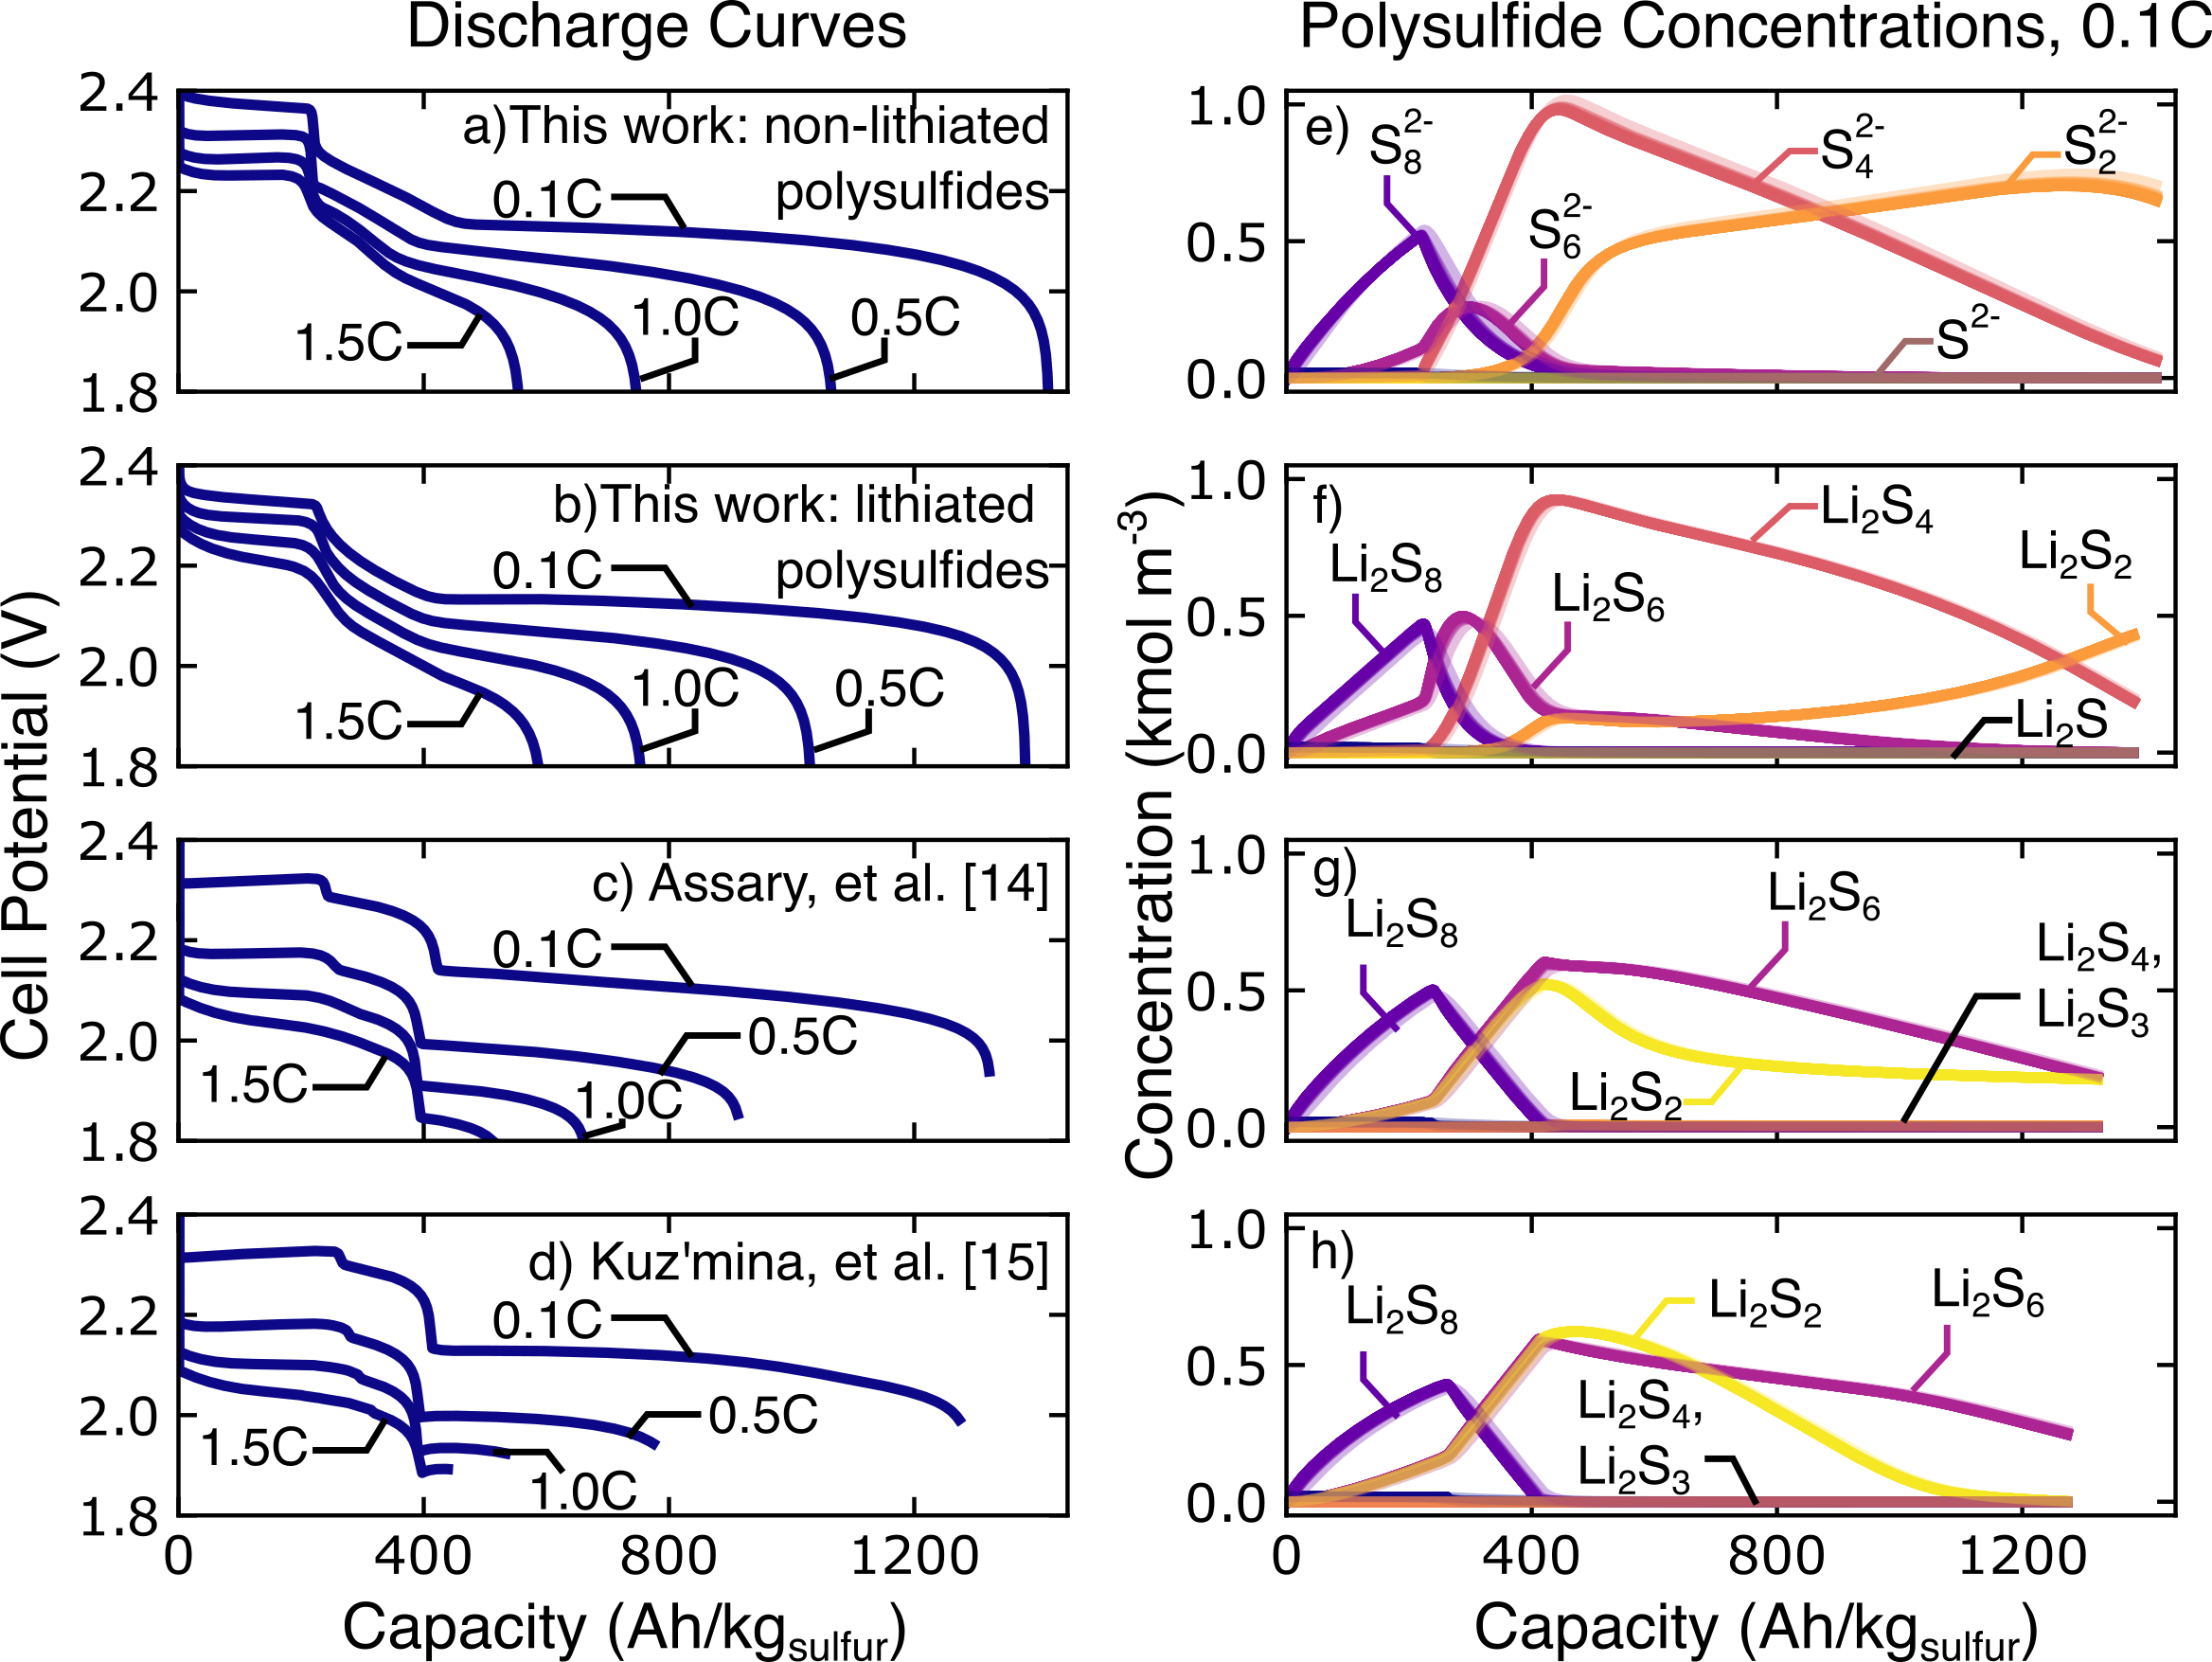
\includegraphics[width=\textwidth]{Figures/Figure3_Mechanism_Comparison.png}
    \caption{Discharge curves (a--d) and polysulfide concentrations (e--h) during discharge for four proposed Li-S mechanisms.  Discharge curves are for rates of 0.1C, 0.5C, 1C and 1.5C with a 65\% porous cathode and 25 $\mu$m separator. Polysulfide concentrations are for discharge at 0.1C. Concentrations are presented for various locations in the cell--lighter shades are closer to the separator/anode interface--but concentration gradients at 0.1C are relatively minor.}
    \label{fig:mechanismcomparison}
\end{figure}
\subsection{Mechanism comparison}
Implementing multiple reaction mechanisms within a common framework allows for direct comparison of mechanism predictions. Figure~\ref{fig:mechanismcomparison} shows discharge curves at rates of 0.1C, 0.5C, 1.0C, and 1.5C (Fig.~\ref{fig:mechanismcomparison}a--d), and dissolved polysulfide molar concentrations (Fig.~\ref{fig:mechanismcomparison}e--h) at a discharge rate of 0.1C  for all four mechanisms. Results demonstrate that the discharge curve alone is not a sufficient indicator of the underlying physio-electro-chemical phenomena.  While the two continuum-derived models (`non-lithiated' and `lithiated' polysulfides, a, b, e, and f) reproduce qualitatively similar discharge profiles, the species profiles show qualitatively different behavior, in terms of the dominant species, at several points during discharge.  The non-lithiated mechanism predicts only a small peak in the S$_6^{2-}$ concentration, during the transition between the upper and lower voltage plateaus, while the similar Li$_2$S$_6$ polysulfide is the dominant species predicted by the lithiated mechanism, during this transition.  Toward the end of discharge, the non-lithiated mechanism shows S$_2^{2-}$ as the dominant species for roughly the last quarter of discharge, while it has a much lower concentration in the lithiated mechanism.  $\mathrm{Li}_2\mathrm{S}_6$ is considered to have a relatively high solubility ($\approx$ 6 M \cite{ANDREI2018469}), while $\mathrm{Li}_2\mathrm{S}_2$ is considered to have a negligible solubility, and would almost certainly precipitate out of solution at the concentrations predicted here.  Understanding the intermediate species concentrations during discharge is therefore critical to controlling shuttling and precipitation, and detailed chemical modeling can play a key role in providing guidance in Li-S battery design and operation.

The two atomistic-derived mechanisms in Fig.~\ref{fig:mechanismcomparison} demonstrate that, while such calculations provide valuable input for mechanism development, considerable work is required to `tune' these mechanisms to provide accurate continuum-scale predictions. The mechanisms provide only thermodynamic parameters, requiring fitting of the kinetic parameters.  The best fits show discrepancies, relative to the experimental validation data in Fig.~\ref{fig:model_validation}. At low discharge rates, both mechanisms show a small, instantaneous drop in cell potential, followed by a concave-down transition between the upper and lower voltage plateaus, neither of which are observed in experimental data. At higher discharge rates, both atomistic mechanisms show significant performance losses (lower cell potentials and capacities) which, again, are not characteristic of the experimental data.

Comparing the differences in discharge curve profiles with those in the polysulfide concentrations highlights the need for accurate species thermodynamics. For example, the shape of the discharge curves during the transition between the upper and lower voltage plateau is dictated by the intermediate polysulfide concentrations. Consistent with the qualitatively different discharge curve shapes in this region, we see significantly different species profiles in the atomistic mechanisms (Figs.~\ref{fig:mechanismcomparison}g and~\ref{fig:mechanismcomparison}h), relative to the continuum-derived models in Figs.~\ref{fig:mechanismcomparison}e and~\ref{fig:mechanismcomparison}f. Whereas the two continuum-derived mechanisms predict a transient peak in the $n=6$ polysulfide (i.e., S$_6^{2-}$ and Li$_2$S$_6$), followed by persistent elevated $n=4$ polysulfide concentrations, the two atomistic models predict persistent elevated Li$_2$S$_6$ concentrations and negligible Li$_2$S$_4$. Additionally, while the continuum-derived mechanisms predict a slow, continuous rise in the $n=2$ polysulfides after consumption of the $n=6$ polysulfides, the atomistic mechanisms predict that the Li$_2$S$_2$ concentration rises in tandem with that of Li$_2$S$_6$, and decreases monotonically after the two species reach a peak concentration at a capacity of roughly 400--500 Ah/kg$_{\rm sulfur}$. Finally, the negligible concentrations of the intermediates Li$_2$S$_4$ and Li$_2$S$_3$ help explain the lower maximum capacities predicted by the atomistic mechanisms.  Regardless of the kinetic rate constants, the necessary reactants are simply not present in sufficient concentrations to sustain further discharge currents.   
\begin{figure}[b!]
    \centering
    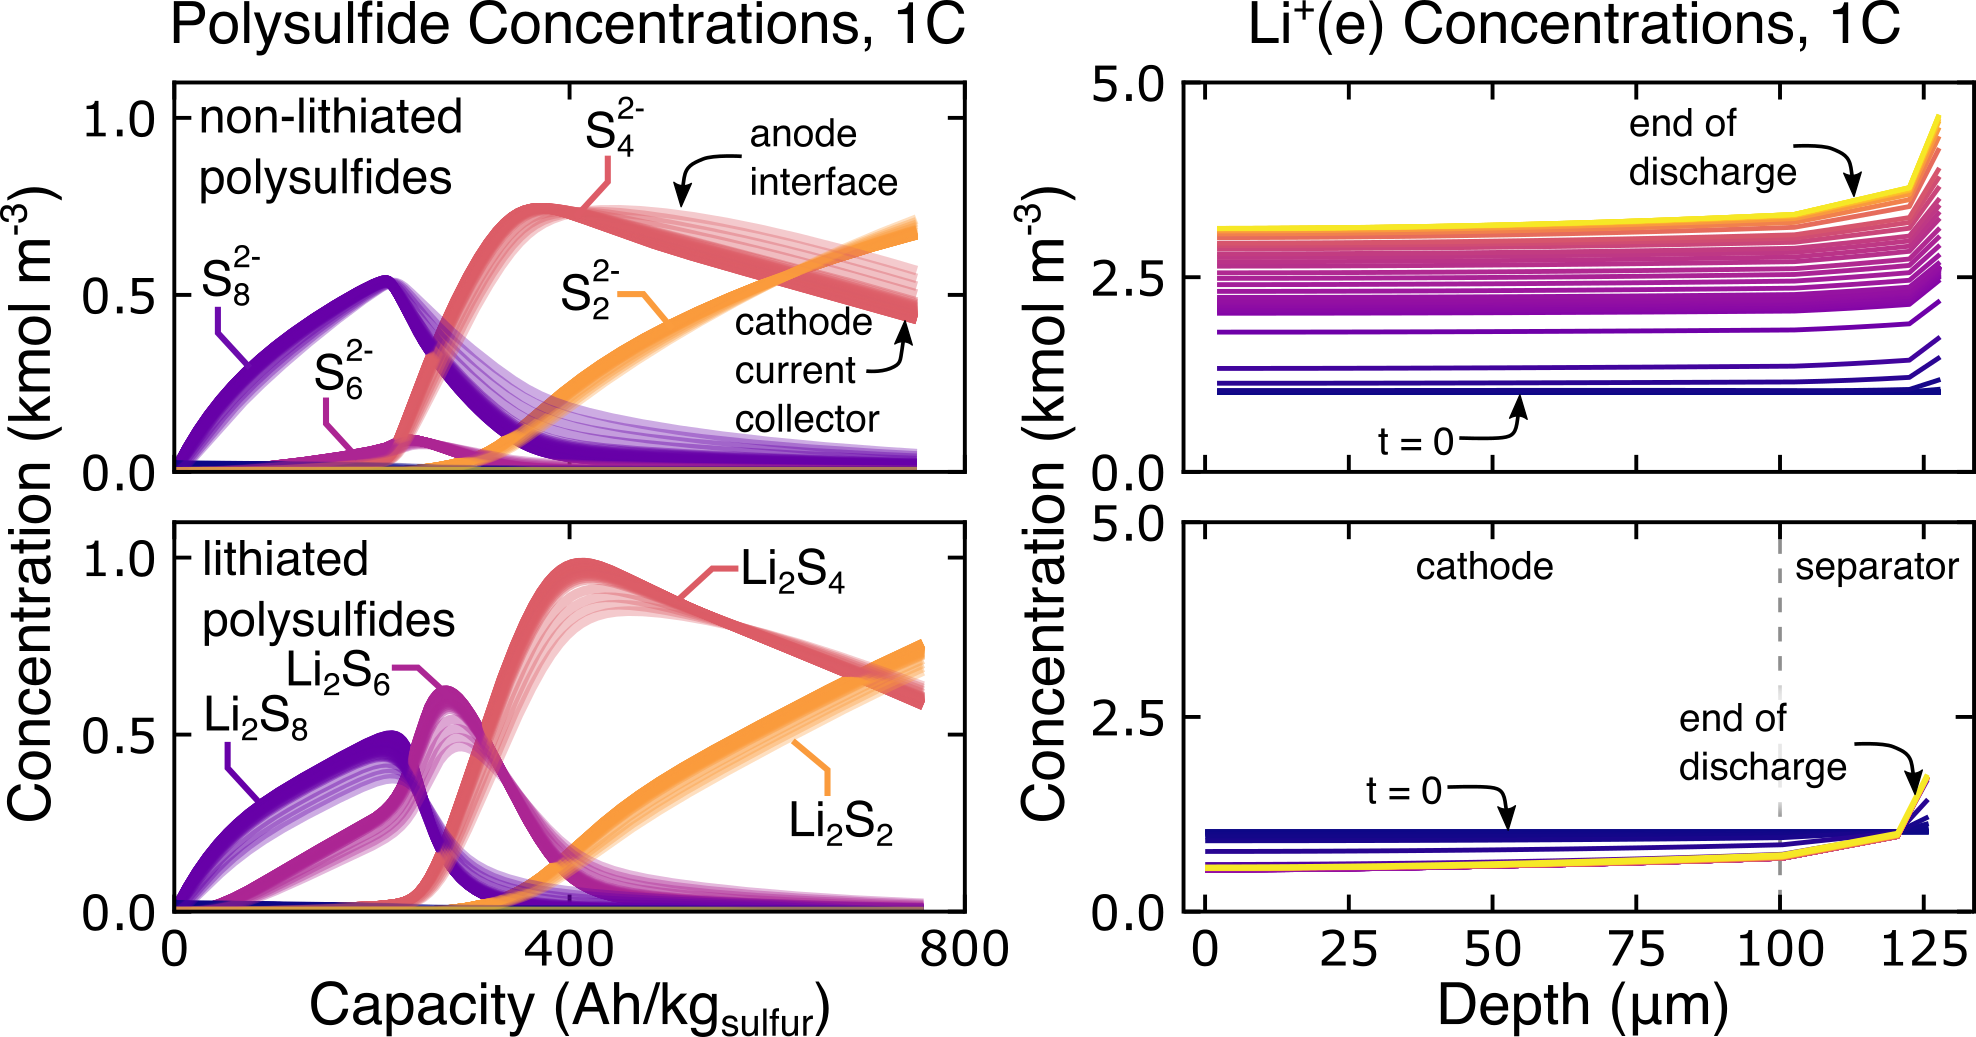
\includegraphics[width=\textwidth]{Figures/Figure4_Polysulfide_Comparison.png}
    \caption{Polysulfide (a,b) and Li$^+$ (c,d) concentrations for the `non-lithiated' and `lithiated' polysulfide mechanisms during discharge at 1C. Polysulfide concentrations are presented as a function of capacity/time, with each trace representing a different location (lighter: closer to the separator/anode interface), while Li$^+$ concentrations are presented as a function of distance from the cathode current collector, with each trace representing a different point in time.}
    \label{fig:mechanismcomparisonconc}
\end{figure}

To better highlight the differences between the lithiated and non-lithiated polysulfide mechanisms, Figure~\ref{fig:mechanismcomparisonconc} shows concentration profiles of polysulfides and Li$^+$ ions for both mechanisms at 1C and an initial cathode porosity of 65\%. Polysulfide concentration profiles as a function of capacity are shown in Figs.~\ref{fig:mechanismcomparisonconc}a and~\ref{fig:mechanismcomparisonconc}b, where each trace shows a different location throughout the cell (darker: near cathode current collector and lighter: near separator/anode interface). For faster discharge, we observe several notable changes in species concentration profiles, relative to 0.1C predictions in Fig.~\ref{fig:mechanismcomparison}. In particular, $n=2$ polysulfide concentrations are now quite similar for the two mechanisms. Also, the S$_6^{2-}$ and  S$_4^{2-}$ concentrations decrease for the non-lithiated mechanism, whereas the  Li$_2$S$_6$ and Li$_2$S$_4$ concentrations increase for the lithiated mechanism, relative to those predicted at 0.1C.

Additionally, as expected, noticeable concentration gradients throughout the cell are predicted at 1C, demonstrating the impact of transport on the two reduction pathways. For both mechanisms, the dynamic evolution of the concentration gradients demonstrates the moderating influence of the electrolyte separator on polysulfide concentrations.  During formation of polysulfides, the concentrations are lower in the separator, as polysulfides move from the cathode toward the anode.  This trend reverses as polysulfides are consumed, and polysulfides diffuse from higher concentration regions in the separator into the cathode. 

There are, however, notable differences in the predicted concentration gradients for the two mechanisms. For the non-lithiated polysulfides, significant concentration gradients occur only during polysulfide consumption, not formation. For the lithiated polysulfides, concentration gradients are observed throughout the discharge process. This is explained by the impact of electric potential on charged polysulfide transport rates. For the the charged S$_n^{2-}$ polysulfides, transport is influenced by both concentration and electric potential gradients, as shown in eq.~\ref{eq:PNP}. During formation, electric potential gradients in the electrolyte promote transport toward the anode, and the formed polysulfides are quickly distributed throughout the cell. When these polysulfide species are later consumed in the cathode, the electric potential gradients impede S$_n^{2-}$ transport from the separator back to the cathode, leading to the observed concentration gradients. For the neutral Li$_2$S$_2$, transport is driven entirely by concentration gradients, and we observe transport-associated concentration gradients throughout the discharge process.

While the polysulfide concentration profiles predicted in Figs.~\ref{fig:mechanismcomparisonconc}a and~\ref{fig:mechanismcomparisonconc}b are qualitatively similar, the $\mathrm{Li}^+$ ion concentrations in Fig.~\ref{fig:mechanismcomparisonconc}c and Fig.~\ref{fig:mechanismcomparisonconc}d are entirely dissimilar.  The figure shows Li$^+$ concentration as a function of distance from the cathode current collector, with each trace representing a different time.  For the non-lithiated polysulfides (Fig.~\ref{fig:mechanismcomparisonconc}c), the Li$^+$ concentration increases throughout the cell, continuously during the discharge process.  For the lithiated polysulfides (Figs.~\ref{fig:mechanismcomparisonconc}d), the average Li$^+$ concentration remains constant; concentration increases at the separator/anode interface are offset by concentration decreases elsewhere.  Moreover, the Li$^+$ concentration profile changes only at the very beginning of the discharge process, quickly reaching a steady state that is maintained throughout the remainder of discharge.

The differences here are explained by the role of Li$^+$ in the discharge process of the two mechanisms. In the non-lithiated form, the $\mathrm{Li}^+$ ions are not required as a reactant for charge transfer reactants, but rather are initially only necessary to maintain charge neutrality with the polysulfide anions S$_\mathrm{n}^{2-}$ formed via reduction in the cathode. The charge added to the electrolyte at the anode/electrolyte interface at every time step is therefore equal and opposite to that added at the cathode/electrolyte interface. Moreover, significant Li$^+$ gradients are only observed toward the end of discharge, when Li$^+$ is consumed in the cathode to form Li$_2$S.  For the lithiated polysulfides, reduction reactions in the cathode consume Li$^+$ to form neutral Li$_2$S$_n$; charged S$_n^{2-}$ are not created.  Hence the total concentration of Li$^+$ cations in the cell remains constant as a function of time, and consumption of Li$^+$ ions in the cathode leads to concentration gradients throughout the discharge process.

Considering the different predictions of these two mechanisms, combined with \textit{operando} polysulfide concentration measurements indicating the presence of lithiated polysulfides,~\cite{SAQIB2017266} we recommend greater incoporation of lithiated polysulfide species in continuum-level simulations, moving forward. As mentioned above, a fully accurate model should eventually incorporate both reaction pathways, but will require significant input from atomistic models and chemically-resolved experimental validation data in order to fit the required parameters. For the remainder of the present work, we use the lithiated polysulfide mechanism to explore advanced battery design.
\begin{figure}[b!]
    \centering
    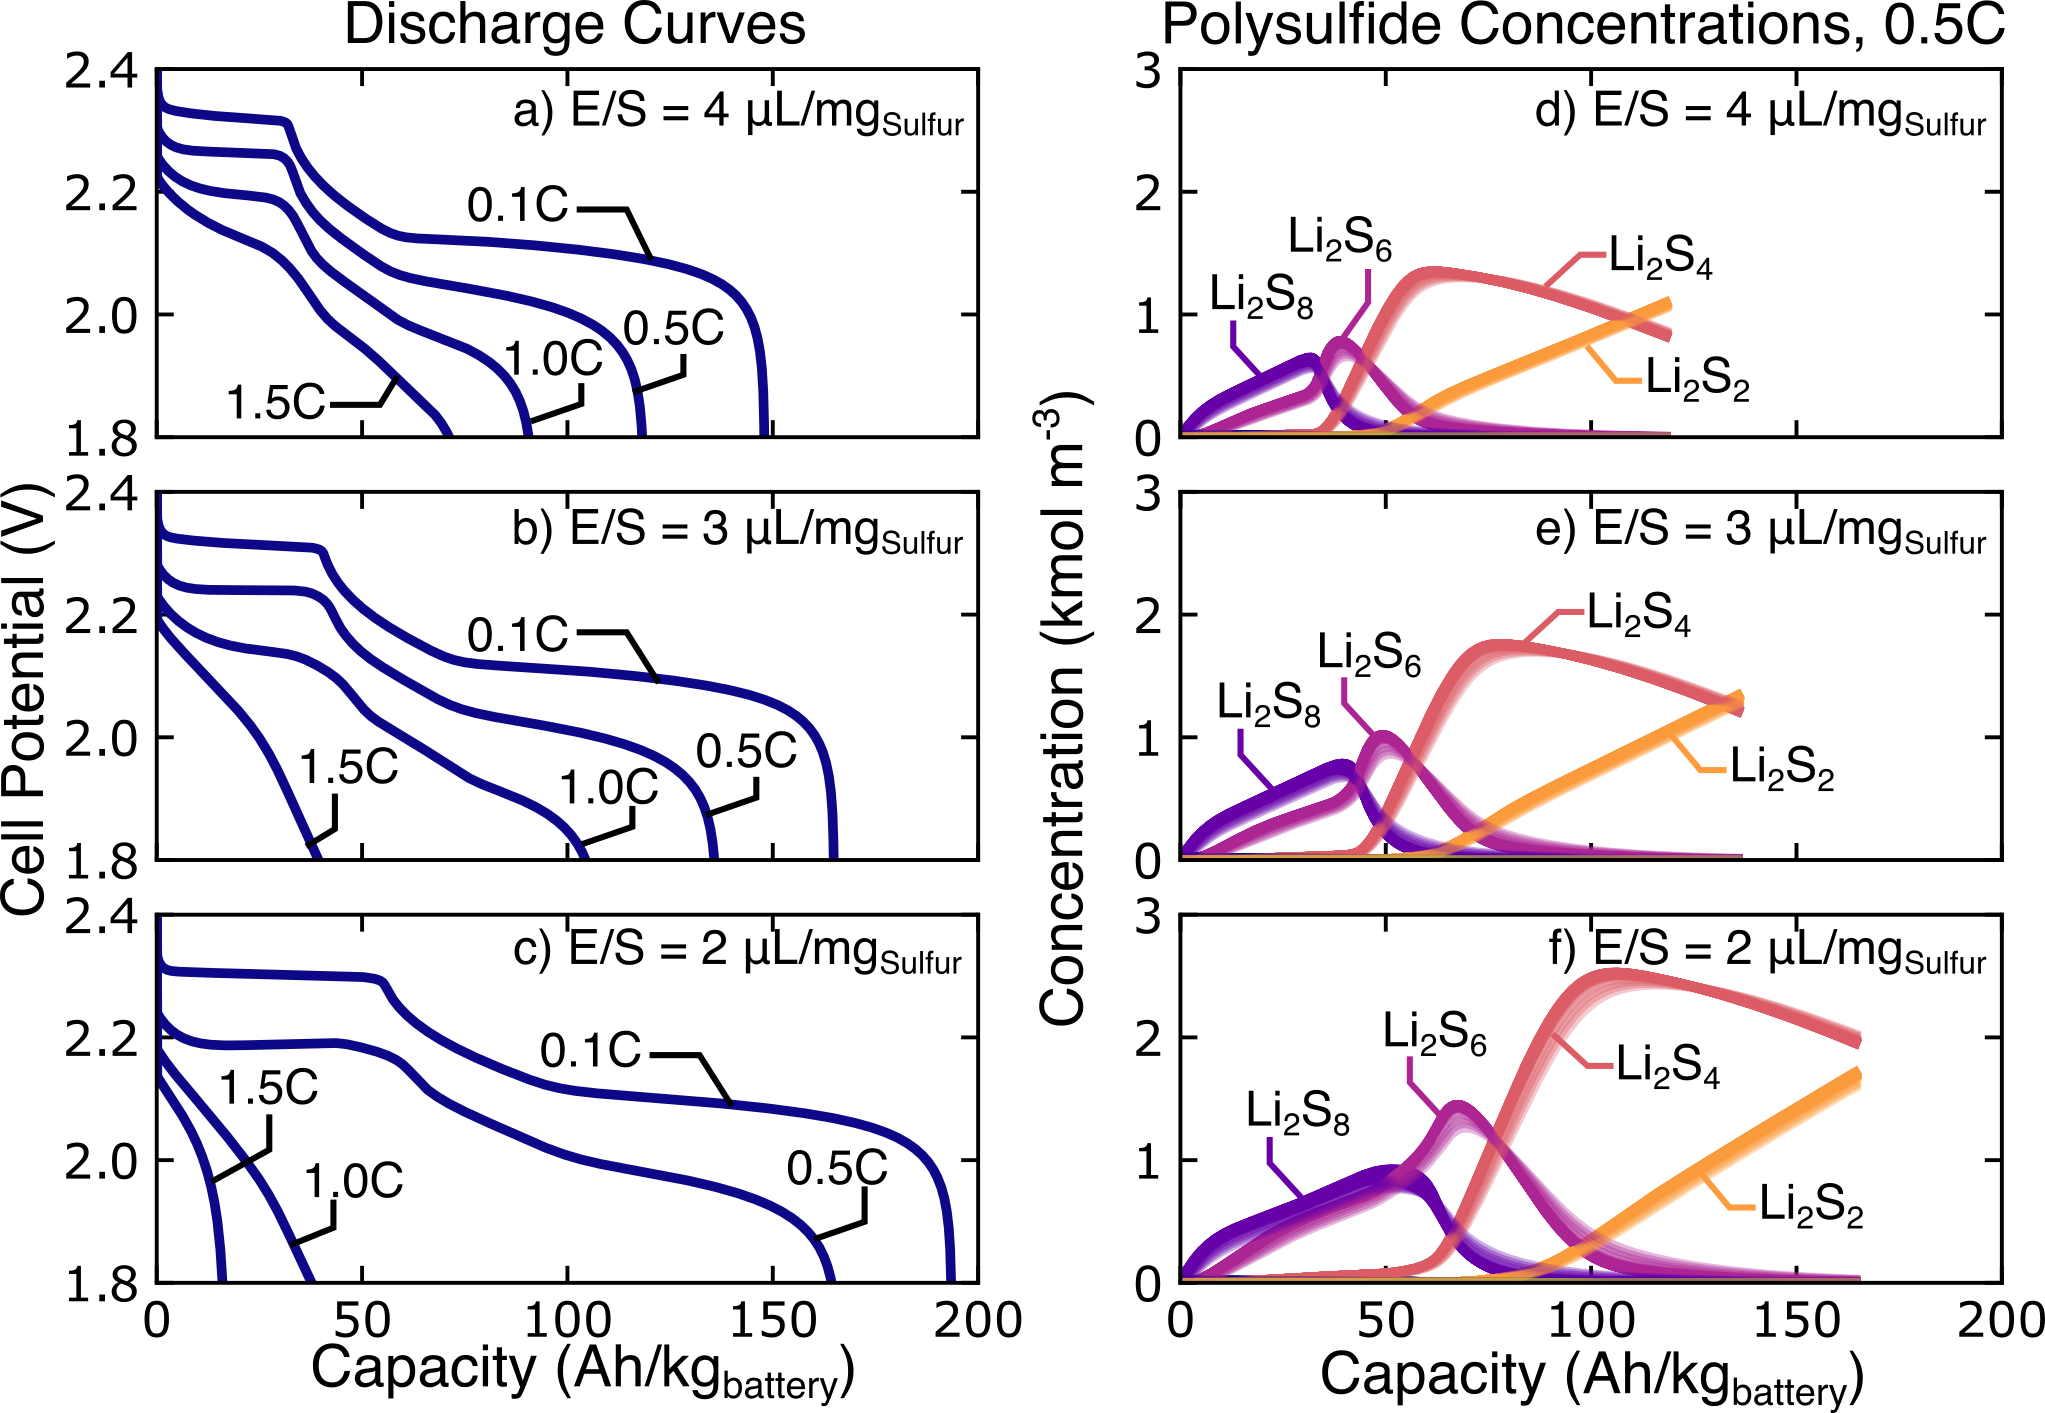
\includegraphics[width=\textwidth]{Figures/Figure5_CellDesign.png}
    \caption{Discharge curves (a--c) and polysulfide concentrations (d--f) for three different electrolyte/sulfur ratios. Discharge curves are presented for 0.1C, 0.5C, 1C, and 1.5C discharge. Species concentrations for each E/S ratio are presented at 0.5C, with each trace representing a different location in the cell (lighter: closer to the electrolyte/anode interface).}
    \label{fig:E_S_ratio_comp}
\end{figure}

\subsection{Cell design}
In order to meet battery performance metrics required for consumer applications, the overall Li-S battery volume and mass must be reduced. This is typically achieved by reducing the volume of electrolyte, per unit mass of sulfur loading, also known as the electrolyte/sulfur (E/S) ratio. Here, we explore the effects of cell design and operation for E/S ratios of 2, 3, and 4 $\mu$L mg$^{-1}_\mathrm{sulfur}$. E/S ratios of 3 $\mu$L mg$^{-1}_\mathrm{sulfur}$ are common in state-of-the-art designs,~\cite{Kang2019} and exploring performance and polysulfide concentrations in the neighborhood of this design can identify performance bottlenecks and degradation pathways and ultimately help inform next-generation battery designs.

%\begin{figure}[t]
%    \centering
%    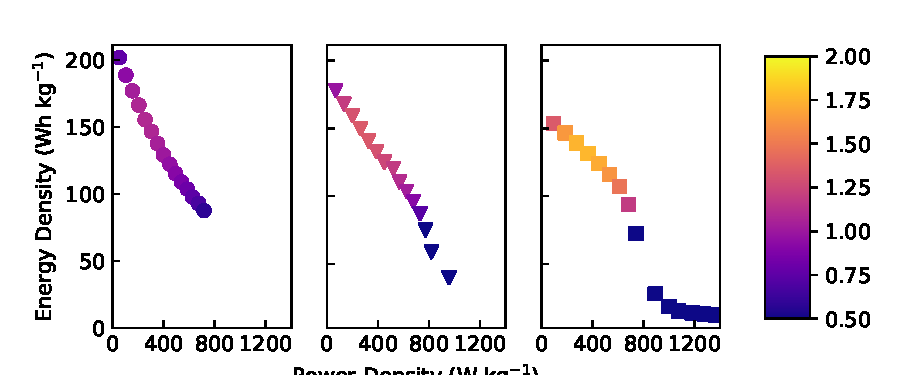
\includegraphics[width=\textwidth]{Figures/Figure7_Ragone_Li2S2.pdf}
%    \caption{Ragone plot showing energy density vs. power density of cells with electrolyte/sulfur ratios of 4 $\mu$L mg$^{-1}$, 3 $\mu$L mg$^{-1}$, and 2 $\mu$L mg$^{-1}$ comparing max concentration reached of Li$_2$S$_2$}
%    \label{fig:ragoneLi2S2}
%\end{figure}

Figures \ref{fig:E_S_ratio_comp}a--\ref{fig:E_S_ratio_comp}c show discharge voltage profiles for the three E/S ratios at 0.1C, 0.5C, 1C, and 1.5C. Note that capacity for these figures is normalized relative to \textit{total} battery mass, whereas the sulfur mass was used for the inquiries in Figs.~\ref{fig:model_validation}--\ref{fig:mechanismcomparisonconc}. As expected, gravimetric discharge capacity increases with decreasing E/S ratio at moderately low C-rates (0.1C and 0.5C), consistent with the decrease in non-active material and therefore battery mass. With increasing C-rate, the lower E/S ratios predict significant losses in performance and capacity, such that the battery with E/S=2~$\mu$L mg$^{-1}_\mathrm{sulfur}$ performs the worst of all E/S ratios at 1.0C and 1.5C. These losses are associated with decreasing porosity with decreasing E/S ratio, which lead to Li$^+$ transport limitations that prevent faster cycling for these batteries.

Figures~\ref{fig:E_S_ratio_comp}d--\ref{fig:E_S_ratio_comp}f show the polysulfide concentrations for all three designs, for discharge at 0.5C.  We observe that the discharge cuts off only moderately earlier, relative to the species availability, at moderate discharge rates. For example, the conversion of Li$_2$S$_4$ to Li$_2$S$_2$ proceeds slightly longer at 4~$\mu$L mg$^{-1}_\mathrm{sulfur}$ than at 2$\mu$L mg$^{-1}_\mathrm{sulfur}$, but not to a degree that outweighs the benefit of reduced inactive material. At higher discharge rates, however, these differences are exacerbated (supplemental Figure S1), and significant concentration gradients are observed throughout the cathode, before premature termination of the discharge process due to Li$^+$ starvation.  

In addition to losses in power and energy performance, Figs.~\ref{fig:E_S_ratio_comp}d--\ref{fig:E_S_ratio_comp}f demonstrate that decreasing E/S ratios increase degradation risks associated with polysulfide precipitation. First, we note that the concentrations increase with decreasing E/S ratio, and are uniformly higher than for Figs.~\ref{fig:mechanismcomparison} and Fig.~\ref{fig:mechanismcomparisonconc}, which were run at an E/S ratio of approximately $5.8 ~ \mu \mathrm{L} ~ \mathrm{mg}^{-1}_\mathrm{sulfur}$. As we see in figure \ref{fig:E_S_ratio_comp}f, the concentration of $\mathrm{Li}_2\mathrm{S}_4$ nearly doubles, exceeding its saturation limit of $\approx$2~kmol m$^{-3}$,~\cite{ANDREI2018469} when the E/S ratio is halved from $4 ~ \mu\mathrm{L} ~ \mathrm{mg}^{-1}_\mathrm{sulfur}$ to $2 ~ \mu\mathrm{L} ~ \mathrm{mg}^{-1}_\mathrm{sulfur}$. These results are consistent with the decreasing total electrolyte volume, and establish that the risk of polysulfide precipitation increases and must be monitored and/or mitigated, with decreasing E/S ratio,

\begin{figure}[b!]
    \centering
    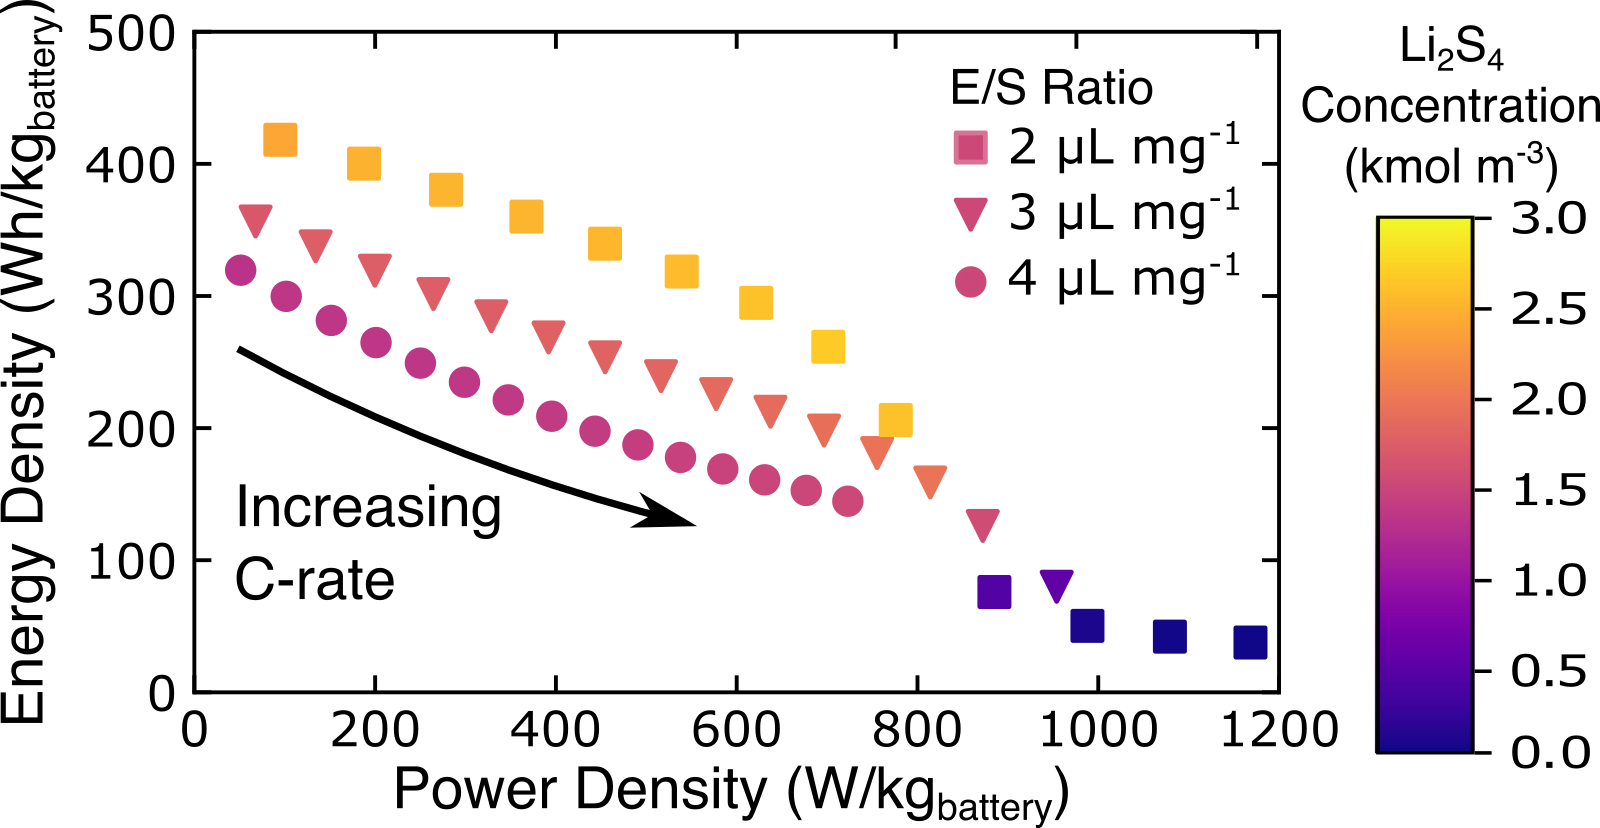
\includegraphics[width=0.85\textwidth]{Figures/Figure6_Li2S4Ragone.png}
    \caption{Ragone plot showing energy density vs. power density of cells with electrolyte/sulfur ratios of 4 $\mu$L mg$^{-1}$, 3 $\mu$L mg$^{-1}$, and 2 $\mu$L mg$^{-1}$ comparing max concentration reached of Li$_2$S$_4$. Discharge rages for all three E/S ratios ranged from 0.1C to 1.5C.}
    \label{fig:ragoneLi2S4}
\end{figure}

The results in Fig.~\ref{fig:E_S_ratio_comp} demonstrate the challenge of balancing performance and longevity in Li-S batteries.  The dominant polysulfide during most of the discharge process is Li$_2$S$_4$ which, as mentioned, has a solubility limit of roughly 2 kmol m$^{-3}$.~\cite{ANDREI2018469}  Figure~\ref{fig:ragoneLi2S4} presents another perspective on this challenge, plotting energy versus power density (i.e. a Ragone plot) for 0.1C to 1.5C discharge, overlaid with a color plot of the max $\mathrm{Li}_2\mathrm{S}_4$ concentration during discharge, for the three E/S ratios considered above. The results show increasing energy density with decreasing E/S, as predicted, up until transport limitations severely hamper the performance of the battery with E/S = $2~\mu\mathrm{L} ~ \mathrm{mg}^{-1}_\mathrm{sulfur}$.  However, we see that the Li$_2$S$_4$ concentration in this lowest E/S cell exceeds its solubility limit for all C-rates where the battery outperforms the other E/S battery designs.  

The cell with E/S = $3~\mu\mathrm{L} ~ \mathrm{mg}^{-1}_\mathrm{sulfur}$, meanwhile, shows a better dynamic performance range than the other designs. The capacity does not suffer the same precipitous losses at high C-rates.  Moreover, this cell maintains Li$_2$S$_4$ concentrations below the solubility limit over the entire range of C-rates and thereby prevents deleterious precipitation phenomena. Given this context, it is understandable that E/S = $3~\mu\mathrm{L} ~ \mathrm{mg}^{-1}_\mathrm{sulfur}$ represents the current state of the art. Advanced designs to further lower E/S will require an approach that not only addresses transport limitations at high power/high C-rate, but also mitigates possible loss of active material due to precipitation of intermediate species.

Considering Li-S battery design more broadly, efforts to mitigate polysulfide shuttling by limiting polysulfide transport out of the cathode (via cation-selective separator coatings, for example), may encounter similar limitations due to the intermediate polysulfide solubility.  Using continuum-level models as a tool to explore the design and operation space of Li-S batteries can therefore provide useful guidance to optimize the battery structure or composition for various applications. Simultaneously, further advances in understanding the intermediate thermo-kinetics in Li-S batteries are required to populate the necessary parameter sets for such detailed chemical modeling. 

%===============================================================%
%                      CONCLUSIONS
%===============================================================%
\section{Conclusions}

In this paper, we present a 1D Li-S battery model which leverages the chemical kinetics software package \textsc{Cantera} to handle thermo-kinetic calculations in a robust, flexible, and generalized manner.  This framework allows for easy comparison of Li-S mechanisms with arbitrary chemical complexity, to better understand and compare the limiting phenomena in each. Given the chemical complexity of Li-S batteries, such a framework provides insight into mechanism aspects needed to capture key features observed experimentally. 

In this study, comparing four different mechanism candidates (two developed as part of this work, two derived from atomistic simulations) to experimental data yields key insights into mechanism development.  For one, the reduction pathway can be written via lithiated or non-lithiated polysulfide intermediates.  Results show that while the two mechanisms can reproduce quite similar discharge curves, they predict qualitatively different polysulfide concentrations and corresponding limiting phenomena. In addition to the overall profiles being different, the two mechanisms predict very different concentration gradients throughout the cell. Spatial gradients in polysulfide concentrations were observed by Miller, \textit{et al} \cite{Miller_2017} using X-ray spectromicroscopy. This type of data could aid in providing further verification of proposed reaction pathways. Due to the differences observed, design decisions based on the two mechanisms might therefore come to entirely different conclusions. While we conclude that a mechanism with purely lithiated polysulfides provides a better match to data than one based on purely non-lithiated polysulfides, ultimately both reaction pathways are likely important for predicting battery performance.~\cite{kamyab2020}

Additionally, the model framework was used to explore the design and limitations of high-performance Li-S batteries via varying E/S ratio for varying discharge rates. The model performance predictions demonstrate the general challenge of balancing high energy and high power density in Li-S batteries.
While low E/S batteries improve the energy density at low C-rates, performance degrades significantly at high C-rates due to Li$^+$ transport limitations, such that only marginal energy density ( $< 100 \mathrm{Wh/kg}$) is recovered at high power.  Moreover, viewing results through the lens of species concentrations demonstrates that polysulfides can readily exceed solubility limits at low E/S ratios, leading to capacity fade due to precipitation of polysulfide intermediates.

This work presents an initial effort to advance the chemical complexity in thermodynamically-reversible Li-S models, but still likely under-represents the actual degree of chemical complexity.  As increasingly complex mechanisms are developed, populating the required model parameters (upwards of 50 thermodynamic and kinetic parameters in the present study) will require input from experiments and theoretical calculations. The challenge of adopting theoretical calculations for continuum-level models should not be dismissed. In this study, we implement two such mechanisms and find that performance and species concentration predictions are qualitatively different from experimental observations. Regardless, the results above demonstrate the value of detailed thermo-chemical modeling for Li-S battery design and analysis. Incorporating parallel lithiated and non-lithiated polysulfide pathways, for example, will likely reduce the predicted polysulfide concentrations, relative to either pathway in isolation.  This, in turn, can help identify favorable battery designs and/or operating strategies for Li-S battery designs that leverage the promise of the chemistry's potential for cheap, portable, efficient, and environmentally benign energy storage.

\section*{Acknowledgements}

This work was authored by Alliance for Sustainable Energy, LLC,
the manager and operator of the National Renewable Energy Laboratory for the U.S. Department of Energy (DOE) under Contract No. DE-AC36-08GO28308. Funding was provided by the U.S. DOE Office of Vehicle Technologies Energy Storage Program, Computer-Aided Engineering of Batteries program manager Brian Cunningham. The views expressed in the article do not necessarily represent the views of the DOE or the U.S. Government. The U.S. Government retains and the publisher, by accepting the article for publication, acknowledges that the U.S. Government retains a nonexclusive, paid-up, irrevocable, worldwide license to publish or reproduce the published form of this work, or allow others to do so, for U.S. Government purposes.

\newpage
\bibliography{mybib}
\newpage



\end{document}